% Document setup
\documentclass[article, a4paper, 11pt, oneside]{memoir}
\usepackage[utf8]{inputenc}
\usepackage[T1]{fontenc}
\usepackage[danish,UKenglish]{babel}

% Formatting
\usepackage[autostyle]{csquotes}
\usepackage[largesmallcaps]{kpfonts}
\usepackage{inconsolata}
\linespread{1.06}
\usepackage[final]{microtype}
\usepackage{xcolor}
\frenchspacing
\let\phi\varphi

% Lists
\usepackage{enumitem}
\setenumerate[0]{label=\normalfont(\arabic*)}

% Bibliography
\usepackage[backend=biber, style=authoryear, maxcitenames=2, useprefix]{biblatex}
\addbibresource{references.bib}

% Mathematics commands
\usepackage{mathtools}
\usepackage{mathcommands}
\numberwithin{equation}{chapter}

% Other commands
\newcommand{\calH}{\mathcal{H}}
\newcommand{\calK}{\mathcal{K}}
\newcommand{\calB}{\mathcal{B}}
\newcommand{\calM}{\mathcal{M}}
\newcommand{\calE}{\mathcal{E}}
\newcommand{\calF}{\mathcal{F}}
\newcommand{\dom}{\mathcal{D}}
\DeclareMathOperator*{\slim}{s-lim}
\newcommand{\symdiff}{\mathbin{\Delta}}
\newcommand{\range}{\mathcal{R}}
\newcommand{\nullspace}{\mathcal{N}}

% Margins
% \setlrmarginsandblock{3cm}{*}{1}
% \checkandfixthelayout

% For list of symbols
\usepackage{longtable,array}

% Index
\usepackage{imakeidx}

% Hyperlinks
\usepackage{hyperref}
\definecolor{linkcolor}{HTML}{4f4fa3}
\hypersetup{%
	pdftitle={Unbounded Operators on Hilbert Space with Applications in Quantum Mechanics},
	pdfauthor={Danny Nygård Hansen},
	colorlinks,
	linkcolor=linkcolor,
	citecolor=linkcolor,
	urlcolor=linkcolor,
	bookmarksnumbered=true
}

% Miscellaneous
\newcommand{\fxnote}[1]{}
%\usepackage[draft]{fixme}
%\usepackage[inline]{showlabels}


%====================================================================
%  FOOTNOTES
%====================================================================

\footmarkstyle{\textsuperscript{#1}\hspace{0.25em}}


%====================================================================
%  THEOREMS
%====================================================================

\usepackage[ntheorem]{mdframed}
\usepackage[amsmath,thmmarks,hyperref]{ntheorem}
\usepackage{thmtools}
\usepackage[capitalize,nameinlink]{cleveref}

% Colours
\definecolor{titlecolor}{HTML}{d6d6f0}
\definecolor{backgroundcolor}{HTML}{ebebf5}

% Framed theorem style
\mdfdefinestyle{swanntheorem}{%
    skipabove=0.5em plus 0.4em minus 0.2em,
	skipbelow=0.5em plus 0.4em minus 0.2em,
	leftmargin=-5pt,
	rightmargin=-5pt,
	innerleftmargin=5pt,
	innerrightmargin=5pt,
	innertopmargin=5pt,
	innerbottommargin=4pt,
	linewidth=0pt,
	splittopskip=1.2em minus 0.2em,
	splitbottomskip=0.5em plus 0.2em minus 0.1em,
	backgroundcolor=backgroundcolor,
	frametitlebackgroundcolor=titlecolor,
	frametitlefont={\scshape},
	theoremtitlefont={\normalfont\itshape},
	frametitleaboveskip=3pt,
	frametitlebelowskip=2pt
}

% Framed theorems
\makeatletter

\mdtheorem[style=swanntheorem, font={\itshape}]{theorem}{\protect\@theorem}[chapter]
\mdtheorem[style=swanntheorem, font={\itshape}]{proposition}[theorem]{\protect\@proposition}
\mdtheorem[style=swanntheorem, font={\itshape}]{lemma}[theorem]{\protect\@lemma}
\mdtheorem[style=swanntheorem, font={\itshape}]{corollary}[theorem]{\protect\@corollary}
\mdtheorem[style=swanntheorem]{definition}[theorem]{\protect\@definition}

\let\oldproposition\proposition
\renewcommand{\proposition}{%
  \crefalias{theorem}{proposition}%
  \oldproposition}

\let\oldlemma\lemma
\renewcommand{\lemma}{%
  \crefalias{theorem}{lemma}%
  \oldlemma}
  
\let\oldcorollary\corollary
\renewcommand{\corollary}{%
  \crefalias{theorem}{corollary}%
  \oldcorollary}

\let\olddefinition\definition
\renewcommand{\definition}{%
  \crefalias{theorem}{definition}%
  \olddefinition}

% https://tex.stackexchange.com/questions/175961/theorem-and-lemma-sharing-counter-with-mdframed-and-cleveref

% Remarks and examples
\newtheoremstyle{myexample}%
  {\item[\hskip\labelsep \theorem@headerfont ##1\ ##2\theorem@separator]}%
  {\item[\hskip\labelsep \theorem@headerfont ##1\ ##2:\ \normalfont##3\theorem@separator]}

\newtheoremstyle{myexamplebreak}%
  {\item[\rlap{\vbox{\hbox{\hskip\labelsep \theorem@headerfont
          ##1\ ##2\theorem@separator}\hbox{\strut}}}]}%
  {\item[\rlap{\vbox{\hbox{\hskip\labelsep \theorem@headerfont
          ##1\ ##2:\ \normalfont##3\theorem@separator}\hbox{\strut}}}]}
\theoremseparator{.}
\theoremheaderfont{\scshape\color{linkcolor}}
\theorembodyfont{\normalfont}
\theoremsymbol{\ensuremath{\lrcorner}}

\theoremstyle{myexample}
\newtheorem{remark}[theorem]{\protect\@remark}
\theoremstyle{myexample}
\newtheorem{example}[theorem]{\protect\@example}

\theoremstyle{myexamplebreak}
\newtheorem{remarkbreak}[theorem]{\protect\@remark}
\theoremstyle{myexamplebreak}
\newtheorem{examplebreak}[theorem]{\protect\@example}




% Proofs
\theoremstyle{nonumberplain}
\theoremsymbol{\ensuremath{\square}}
\newtheorem{proof}{\protect\@proof}

\newtheoremstyle{MyNonumberplain}%
  {\item[\theorem@headerfont\hskip\labelsep ##1\theorem@separator]}%
  {\item[\theorem@headerfont\hskip\labelsep ##3\theorem@separator]}
\theoremstyle{MyNonumberplain}
\theorembodyfont{\upshape}
\newtheorem{proofof}{Proof}
% https://tex.stackexchange.com/questions/106072/proof-titles-with-ntheorem


%====================================================================
%  THEOREM LIST EXPERIMENT
%====================================================================

% https://tex.stackexchange.com/a/336213/63353

\newcommand{\enumformat}{(\roman*)}
\newcommand{\enumsubformat}[1]{(\roman{#1})}

\newcounter{subcreftmpcnt} %
\newcommand\alphsubformat[1]{(\alph{#1})} %adapt ....
\newcommand\subcref[2][\enumsubformat]{%
\ifcsname r@#2@cref\endcsname
  \cref@getcounter {#2}{\mylabel}%
  \setcounter{subcreftmpcnt}{\mylabel}%
  \hyperref[#2]{\enumsubformat{subcreftmpcnt}}%
 \else ?? \fi}


\newcommand{\mynameref}[2]{%
    \hyperref[#1]{#2~\labelcref*{#1}}%
}

\newlist{enumthm}{enumerate}{1} % a dedicated enum. env.
\setlist[enumthm]{label=\upshape\enumformat, ref=\upshape\thetheorem\enumformat}
\crefalias{enumthmi}{theorem}

\newlist{enumprop}{enumerate}{1} % a dedicated enum. env.
\setlist[enumprop]{label=\upshape\enumformat, ref=\upshape\thetheorem\enumformat}
\crefalias{enumpropi}{proposition}

\newlist{enumcor}{enumerate}{1} % a dedicated enum. env.
\setlist[enumcor]{label=\upshape\enumformat, ref=\upshape\thetheorem\enumformat}
\crefalias{enumcori}{corollary}

\newlist{enumlem}{enumerate}{1} % a dedicated enum. env.
\setlist[enumlem]{label=\upshape\enumformat, ref=\upshape\thetheorem\enumformat}
\crefalias{enumlemi}{lemma}

\newlist{enumdef}{enumerate}{1} % a dedicated enum. env.
\setlist[enumdef]{label=\upshape\enumformat, ref=\upshape\thetheorem\enumformat}
\crefalias{enumdefi}{definition}


%====================================================================
%  REFERENCES
%====================================================================

% Theorems
\Crefname{theorem}{\protect\@theorem}{\protect\@theorempl}
\Crefname{proposition}{\protect\@proposition}{\protect\@propositionpl}
\Crefname{lemma}{\protect\@lemma}{\protect\@lemmapl}
\Crefname{corollary}{\protect\@corollary}{\protect\@corollarypl}
\Crefname{definition}{\protect\@definition}{\protect\@definitionpl}
\Crefname{remark}{\protect\@remark}{\protect\@remarkpl}
\Crefname{example}{\protect\@example}{\protect\@examplepl}
% Only defining \Crefname variants automatically defines \crefname variants with initial letter
% lower case. Use the optional parameter 'capitalise' when importing cleveref to capitalise it
% automatically.

% Sections
\Crefname{chapter}{Section}{Sections}
\Crefname{section}{Subsection}{Subsections}

% Equations
\crefformat{equation}{(#2#1#3)}


%====================================================================
%  LANGUAGES
%====================================================================

% Theorem names, singular
\newcommand{\@theorem}{}
\newcommand{\@proposition}{}
\newcommand{\@corollary}{}
\newcommand{\@lemma}{}
\newcommand{\@definition}{}
\newcommand{\@example}{}
\newcommand{\@remark}{}
\newcommand{\@proof}{}

% Theorem names, plural
\newcommand{\@theorempl}{}
\newcommand{\@propositionpl}{}
\newcommand{\@corollarypl}{}
\newcommand{\@lemmapl}{}
\newcommand{\@definitionpl}{}
\newcommand{\@examplepl}{}
\newcommand{\@remarkpl}{}
\newcommand{\@proofpl}{}

\addto\captionsUKenglish{%
	\renewcommand{\@theorem}{Theorem}%
	\renewcommand{\@proposition}{Proposition}%
	\renewcommand{\@corollary}{Corollary}%
	\renewcommand{\@lemma}{Lemma}%
	\renewcommand{\@definition}{Definition}%
	\renewcommand{\@example}{Example}%
	\renewcommand{\@remark}{Remark}%
	\renewcommand{\@proof}{Proof}%
	%
	\renewcommand{\@theorempl}{Theorems}%
	\renewcommand{\@propositionpl}{Propositions}%
	\renewcommand{\@corollarypl}{Corollaries}%
	\renewcommand{\@lemmapl}{Lemmata}%
	\renewcommand{\@definitionpl}{Definitions}%
	\renewcommand{\@examplepl}{Examples}%
	\renewcommand{\@remarkpl}{Remarks}%
	\renewcommand{\@proofpl}{Proofs}%
}
\addto\captionsdanish{%
	\renewcommand{\@theorem}{Sætning}%
	\renewcommand{\@proposition}{Proposition}%
	\renewcommand{\@corollary}{Korollar}%
	\renewcommand{\@lemma}{Lemma}%
	\renewcommand{\@definition}{Definition}%
	\renewcommand{\@example}{Eksempel}%
	\renewcommand{\@remark}{Bemærkning}%
	\renewcommand{\@proof}{Bevis}%
	%
	\renewcommand{\@theorempl}{Sætninger}%
	\renewcommand{\@propositionpl}{Propositioner}%
	\renewcommand{\@corollarypl}{Korollarer}%
	\renewcommand{\@lemmapl}{Lemmaer}%
	\renewcommand{\@definitionpl}{Definitioner}%
	\renewcommand{\@examplepl}{Eksempler}%
	\renewcommand{\@remarkpl}{Bemærkninger}%
	\renewcommand{\@proofpl}{Beviser}%
}

\makeatother


%====================================================================
%  SECTION TITLES
%====================================================================

% Fleurons
\usepackage{adforn}

% Chapter style
\makechapterstyle{mychapter}{
    \renewcommand{\chapnamefont}{\centering\normalfont} 
    \renewcommand{\chapnumfont}{\centering\normalfont\itshape} 
    \renewcommand\chaptitlefont{\centering\LARGE\normalfont}
    \renewcommand{\printchaptername}{}
    \renewcommand{\chapternamenum}{}
    %\renewcommand{\printchapternum}{\chapnumfont \adfflatleafoutlineleft~~\thechapter~~\adfflatleafoutlineright}
    \renewcommand{\printchapternum}{\chapnumfont ---~~\thechapter~~---}
    \renewcommand*{\afterchapternum}{\par\nobreak\midchapskip}
}

\chapterstyle{mychapter}

% Section titles
\setsecheadstyle{\normalfont\Large\itshape}
\setsecnumformat{\csname the#1\endcsname~~{\normalsize\textbullet}~~}

%====================================================================
%  PAGESTYLE
%====================================================================

\makeatletter

%\renewcommand*{\memUChead}[1]{\MakeTextLowercase{#1}}
\nouppercaseheads

\makepagestyle{thesis}
\makeoddhead  {thesis} {\small\itshape\rightmark} {} {\small\itshape\thepage}
\makeoddfoot  {thesis} {}{}{}
\makepsmarks  {thesis}{
	\createmark{chapter}    {both} {shownumber} {} {. \ }
	\createmark{section}    {right}{shownumber} {}            {. \ }
	\createplainmark{toc}   {both} {\contentsname}
	\createplainmark{lof}   {both} {\listfigurename}
	\createplainmark{lot}   {both} {\listtablename}
	\createplainmark{bib}   {both} {\bibname}
	\createplainmark{index} {both} {\indexname}
}

\pagestyle{thesis}

\makeatother

%====================================================================
%  FRONT PAGE
%====================================================================

\makeatletter
\renewcommand{\maketitle}{
\begin{titlingpage*}
	% Front page
	\calccentering{\unitlength}
	\begin{adjustwidth*}{\unitlength}{-\unitlength}
		\begin{adjustwidth}{-0.5cm}{-0.5cm}
		\centering
		\thispagestyle{empty}
		{%
			\large%
			{\LARGE Unbounded Operators on Hilbert Space \\ with Applications in Quantum Mechanics}\par
			\vspace*{0.5\onelineskip}%
			------\par%\adfflatleafoutlineleft\par
			\vspace*{0.5\onelineskip}%
			{\itshape Ubegrænsede operatorer på Hilbertrum \\ med anvendelser i kvantemekanik}\par
			\vspace*{4\onelineskip}\par
			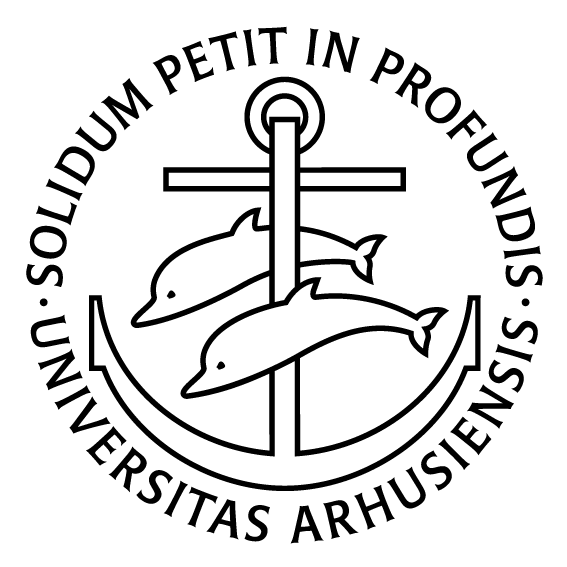
\includegraphics[width=8cm]{ausegl_sort.png}\par
			\vspace*{4\onelineskip}%
			Bachelor Project in Mathematics\par
			Danny Nygård Hansen~~{\footnotesize\textbullet}~~201605113\par
		}%
		\vfill
		\vspace*{2\onelineskip}
		Supervisor: Erik Skibsted\hfill
		January 2021\par
		\vspace*{2\onelineskip}%
		\small%
		Department of Mathematics\par
		Aarhus University\par~\par
		%\emph{Må gerne offentliggøres}%
		\enlargethispage{2\onelineskip}
		\end{adjustwidth}
	\end{adjustwidth*}
	\newpage
	%
	% Colophon
    \thispagestyle{empty}
    \small%
    \strut\vfill
    \begin{flushleft}
    	\copyright\ Danny Nygård Hansen 2021 \par
    	Layout and typography by the author \par
    	Font: 11\,pt Kp-fonts\par% | \texttt{Inconsolata} \par
    	Typeset using \textsc{pdf}\LaTeX{} and the \emph{memoir} class \par
    \end{flushleft}
    \newpage
\end{titlingpage*}
}

%====================================================================
%  TABLE OF CONTENTS
%====================================================================

\renewcommand*{\cftchapterleader}{}
\renewcommand*{\cftsectionleader}{}
\renewcommand{\cftchapterpagefont}{}
\renewcommand*{\cftchapterformatpnum}[1]{\itshape~~{\footnotesize\textbullet}~~#1}
\renewcommand*{\cftsectionformatpnum}[1]{\itshape~~{\footnotesize\textbullet}~~#1}
\renewcommand{\cftchapterafterpnum}{\cftparfillskip}
\renewcommand{\cftsectionafterpnum}{\cftparfillskip}

% I'm trying to redefine chapter/section numberings to get a small caps minuscule letter for appendices.
% Is it smart to redefine this stuff???
% And is that really what I want? It looks fine in headers!
\renewcommand*{\numberline}[1]{%
  \numberlinehook{#1}%
  \hb@xt@\@tempdima{\@cftn@me\@cftbsnum {#1}\@cftasnum\hfil}\@cftasnumb}
\renewcommand{\chapternumberline}[1]{%
  \chapternumberlinehook{#1}%
  \hb@xt@\@tempdima{\@chapapp@head\@cftbsnum {#1}\@cftasnum\hfil}%
  \@cftasnumb}

\renewcommand{\cftchapterpagefont}{\normalfont\large} % Chapter page numbers
\renewcommand{\cftchapterfont}{\normalfont\large} % Chapter title and number
\setlength{\cftbeforesectionskip}{3pt}
\setrmarg{3.55em plus 1fil}

\makeatother

%====================================================================
%  END PREAMBLE
%====================================================================

\makeindex[intoc]

\begin{document}

\frontmatter

\maketitle

\begin{otherlanguage}{danish}
\begin{abstract}
    \noindent I denne opgave udvikler vi den basale teori for selvadjungerede operatorer på Hilbertrum og anvender den på adskillige fundamentale eksempler på operatorer som optræder i kvantemekanikken.
    
    Vi antager kendskab til begrænsede operatorer og beviser en spektralsætning for en ubegrænset selvadjungeret operator. Vi betragter stærkt kontinuerte énparameter unitære grupper og beviser Stones sætning som giver en karakterisation af disse grupper. Vi ser da på multiplikations- og differentialoperatorer, beviser selvadjungerethed og beregner spektre for generelle klasser af disse slags operatorer.
    
    Til sidst betragter vi positions- og potentialoperatorer, samt impuls- og kinetisk energioperatorer. Vi ser især på sidstnævnte, idet vi udleder tidsudviklingen for en fri partikel.
\end{abstract}
\end{otherlanguage}
\begin{abstract}
    \noindent In this thesis we develop the basic theory of self-adjoint operators on Hilbert space and apply it to several fundamental examples of operators appearing in quantum mechanics.
    
    Assuming knowledge of bounded operators, we prove a spectral theorem for an unbounded self-adjoint operator. We consider strongly continuous one-parameter unitary groups and prove Stone's theorem, which gives a characterisation of these groups. We then consider multiplication and differential operators, proving self-adjointness and calculating spectra for general classes of these types of operators.
    
    Finally we consider the position and potential operators, as well as momentum and kinetic energy operators. We pay particular attention to the latter, deriving the time-evolution of a free particle.
\end{abstract}

\newpage

\tableofcontents
\newpage

\newcommand{\borel}{\mathfrak{B}}
\newcommand{\measurable}{\mathcal{M}}
\newcommand{\simplemeas}{\mathcal{S\!M}}
\newcommand{\boundedop}{\mathcal{B}}
\newcommand{\graph}{\mathcal{G}}

\newcommand{\unitary}{\mathrm{U}}
\newcommand{\contcpt}{C_c}
\newcommand{\smoothcpt}{C^\infty_c}
\newcommand{\smoothinf}{C^\infty_0}

\newcommand{\symbolheader}[1]{\multicolumn{2}{l}{\textit{#1}}}

\chapter{Preface}

Until the turn of the twentieth century classical mechanics enjoyed great success, both experimentally and theoretically, the latter in particular in the analytical mechanics due to Lagrange and Hamilton. The end of the nineteenth century saw Planck solve the so-called \textquote{ultraviolet catastrophe} by quantising the exchange of energy in the interaction of matter with electromagnetic radiation, ushering in a new era of physics: quantum mechanics. This development continued in the early 1900s with advances by Einstein, Bohr, Heisenberg and others.

This was paralleled by foundational work in the late 1920s attempting to develop a rigorous mathematical foundation for quantum mechanics. Hilbert spaces and unbounded operators take centre stage, and the systematic development of these operators are first and foremost due to \textcite{vonneumann1930} and \textcite{stone1932a}.

In this thesis we develop some of this theory. In particular, we prove a spectral theorem for unbounded self-adjoint operators and a theorem due to Stone which characterises certain groups of unitary operators in terms of exponential functions. We then apply these to the Schrödinger equation, after which we consider some of the most important operators in quantum mechanics, prove their self-adjointness and calculate their spectra. We focus on the kinetic energy operator, deriving the time-evolution of a free particle. An attempt has been made to be as general as possible without detracting from the main goal, which is the application of these theorems in quantum mechanics.

We assume knowledge of measure theory and functional analysis as seen in the course Advanced Analysis at Aarhus University, roughly at the level of \textcite{rudinfunctional}. In particular, it is assumed that the reader knows the basic theory of bounded operators on Hilbert space and fundamental theorems such as the Hahn--Banach theorem. Prerequisites not explicitly covered in this course or bachelor courses at Aarhus University, such as the $d$-dimensional Fourier transform and the Baire category theorem, are collected in an appendix. We either prove all claims or explicitly refer to the literature. A passing familiarity with quantum mechanics would also be beneficial to appreciate the material, but should not be strictly necessary.

For the general theory of unbounded operators the main references have been \textcite{rudinfunctional}, \textcite{schmudgen2012} and the notes \textcite{skibsted2003}. For applications in quantum mechanics as well as historical notes I have greatly benefited from \textcite{reedsimon2} and \textcite{hall2013}. \textcite{sakurai2011} has been my go-to for the physicist's perspective. The texts \textcite{rudinrealcomplex} and in particular \textcite{folland2007} have also been very useful as general references.

It is a pleasure to give a thanks first of all to Erik Skibsted for an inspiring course in Advanced Analysis, and for his effective guidance while writing this thesis. Also a thank you to Steen Thorbjørnsen for teaching me analysis, and to Søren Fournais for introducing me to mathematical physics.

~

\noindent The layout and typography of the present thesis were implemented by myself, but much has been borrowed from Steen Thorbjørnsen's wonderful (both in content and in style) \emph{Grundlæggende mål- og integralteori}. I also owe a great debt to Lars Madsen, whose \emph{Introduktion til \LaTeX} has been a tremendous help and source of inspiration over the years.

Definitions and theorems are placed in coloured boxes to set them apart from the surrounding text. Note that these boxes may span multiple pages. Following common practice, we use the tombstone \textquote{$\square$} to denote the end of a proof. Examples and remarks are terminated with a \textquote{$\lrcorner$}.

\vspace{\baselineskip}

\noindent Aarhus, January 2021 \hfill Danny Nygård Hansen


\mainmatter

% \section{Notation}

% For a topological space $X$, we denote the Borel $\sigma$-algebra on $X$ by $\borel(X)$. If $(X, \calE)$ is a measurable space, we use $\measurable(\calE)$ to denote the algebra of complex-valued $(\calE, \borel(\setC))$-measurable functions, and we denote by $\simplemeas(\calE)$ the subalgebra of $\measurable(\calE)$ consisting of simple functions. The algebra\fxnote{Or just vector space?} of continuous functions on $X$ with compact support is denoted $\contcpt(X)$, and we write $\smoothcpt(\setR)$ for the algebra of smooth functions on $\setR$ with compact support.

% For a normed vector space $X$, the vector space of bounded operators on $X$ is denoted $\boundedop(X)$. The range of a linear map $T$ will be denoted $\range(T)$ and its kernel $\nullspace(T)$. We write $\graph(T)$ for the graph of $T$.

% If $X$ is an inner product space, we denote the inner product $\inner{\,\cdot\,}{\,\cdot\,}_X$. If no confusion arises, we also omit the subscript $X$. Our inner products are linear in the first entry. The notation $\unitary(\calH)$ is used for the group of unitary operators on a Hilbert space $\calH$.

% The integral of a Lebesgue-measurable function $f$ on the domain $A \subseteq \setR$ is denoted $\int_A f(t) \dif t$.

% If $(\Omega, \calE)$ is a measurable space and $E$ is a spectral measure (cf. \cref{sec:spectral_measures}) on $\calE$, $\calL^\infty(E)$ denotes the space of functions that are essentially bounded with respect to $E$.\footnote{See \textcite[Section~3.4]{skibsted2019} for details.}

% If $X$ is a set and $A \subseteq X$ a subset, $\indicator{A} \colon X \to \{0,1\}$ denotes the indicator function (or characteristic function) on $A$.


\chapter{Unbounded operators}

\section{Definitions and examples}

\begin{definition}
    If $X$ and $Y$ are vector spaces, an \emph{operator}\index{operator} from $X$ to $Y$ is a linear map $T$ from a subspace of $X$ into $Y$. This subspace is called the \emph{domain}\index{operator!domain} of $T$ and is denoted $\dom(T)$. If $T$ is an operator from $X$ to $Y$, we also write $T\colon X \to Y$.
\end{definition}
%
The spaces $X$ and $Y$ will always be normed, and to emphasise that an operator $T$ is not necessarily bounded, we will sometimes call such an operator \emph{unbounded}\index{operator!unbounded}, although a better name might have been \emph{not necessarily bounded}.

Our motivation for introducing unbounded operators is that many of the operators appearing in quantum mechanics (and physics more broadly) are unbounded. An important class of operators is the class of differential operators, illustrated by the following simple example:
%
\begin{examplebreak}[An unbounded differential operator]
    Equip $C[0,1]$ with the supremum norm, and let $T \colon C[0,1] \to C[0,1]$ be the differential operator $Tf = f'$ with domain $\dom(T) = C^1[0,1]$. This is clearly well-defined and linear. But consider the sequence of functions $(f_n)$ given by $f_n(x) = \e^{\iu nx}$. Then $\norm{f_n}_\infty = 1$, but $\norm{Tf_n}_\infty = n$, so $T$ is not bounded on its domain.
\end{examplebreak}
%
The operator in the example above is not defined everywhere on $C[0,1]$. However, there do exist operators that are everywhere-defined but not bounded, as the following example shows:
%
\begin{examplebreak}[An everywhere-defined not bounded operator]
    Let $X$ be an infinite-dimensional normed space, and let $Y \neq 0$ be a normed space. Choose a Hamel basis $\calB$ for $X$, and let $\calB' = \set{b_n}{n \in \setN}$ be a countable subset of $\calB$. Pick some $y \in Y$ with $y \neq 0$. Then define
    %
    \begin{equation*}
        T(b) =
        \begin{cases}
            n \norm{b_n} y, & b = b_n, \\
            0, & b \in \calB \setminus \calB',
        \end{cases}
    \end{equation*}
    %
    and extend $T$ to an operator on $X$. Then $T \colon X \to Y$ is clearly everywhere-defined and not bounded.
\end{examplebreak}

If $S,T \colon X \to Y$ are operators with $\dom(S) \subseteq \dom(T)$ such that $Sx = Tx$ for all $x \in \dom(S)$, then we write $S \subseteq T$ and say that $T$ is an \emph{extension}\index{operator!extension} of $S$. This is clearly equivalent to the condition $\graph(S) \subseteq \graph(T)$, where $\graph(T)$ denotes the graph of an operator $T$.

Since operators are not necessarily defined on the whole space, one must take care when e.g. adding or composing operators. We refer the reader to \textcite[Definitions~13.1]{rudinfunctional} or \textcite[Section~1.1.1]{schmudgen2012} for details. Furthermore, note that for an operator $T \colon \calH \to \calK$ between Hilbert spaces\footnote{More generally from a Hilbert space into a Banach space.} that is bounded on $\dom(T)$, we can always extend it to $\calH$: First extend it to $\closure{\dom(T)}$ using the \mynameref{thm:blt}{BLT Theorem}, and then let $Tx = 0$ for $x \in \closure{\dom(T)}^\perp$.

An important class of operators are the \emph{closed operators}:

\begin{definition}[Closed and closable operators]
    An operator $T \colon X \to Y$ between normed spaces is \emph{closed}\index{operator!closed} if its graph $\graph(T)$ is a closed subset of the direct sum $X \oplus Y$. Furthermore, $T$ is \emph{closable}\index{operator!closable} if the closure of its graph is the graph of some function. The function corresponding to $\closure{\graph(T)}$ is called the \emph{closure}\index{operator!closure} of $T$ and is denoted $\closure{T}$.
\end{definition}
%
If $\closure{\graph(T)}$ is the graph of a function, that function is clearly an operator $\closure{T}\colon X \to Y$ since $\closure{\graph(T)}$ is a subspace of $X \oplus Y$. If $X$ and $Y$ are Banach spaces, it follows from the \mynameref{thm:closed_graph}{Closed Graph Theorem} that $T \in \boundedop(X,Y)$ if and only if $\dom(T) = X$ and $T$ is closed.


\begin{definition}[Spectrum and resolvent of an operator]
    An operator $T \colon X \to Y$ between Banach spaces is \emph{boundedly invertible}\index{operator!boundedly invertible} if there is a bounded operator $S \colon Y \to X$ such that $TS = 1$ and $ST \subseteq 1$. The \emph{resolvent set $\rho(T)$}\index{operator!resolvent set} of $T$ is the set of complex numbers $\lambda$ such that $\lambda - T$ is boundedly invertible. The \emph{spectrum}\index{operator!spectrum} of $T$ is the set $\sigma(T) = \setC \setminus \rho(T)$.
\end{definition}
%
Note that the \mynameref{thm:bounded_inverse}{Bounded Inverse Theorem} ensures that this definition of the spectrum agrees with that of a bounded operator if $T \in \boundedop(X,Y)$.

In the sequel, we will restrict to operators between Hilbert spaces, and the symbols $\calH$ and $\calK$ will denote arbitrary Hilbert spaces.



\section{Symmetric and self-adjoint operators}

Let $T \colon \calH \to \calK$ be an operator. We wish to associate an adjoint operator $T^* \colon \calK \to \calH$ to $T$. First let $\dom(T^*)$ be the set of all $y \in \calK$ such that the linear functional $x \mapsto \inner{Tx}{y}$ is continuous on $\dom(T)$. If $y \in \dom(T^*)$, then the Hahn--Banach theorem extends the above functional to a continuous linear functional $\phi \colon \calH \to \setC$.\footnote{Alternatively, the \mynameref{thm:blt}{BLT Theorem} extends the functional to a bounded linear functional on the closed subspace $\overline{\dom(T)}$, and we may then extend it to $\calH$ using the projection theorem.} The Riesz--Fréchet theorem then yields an element $y_\phi \in \calH$ such that $\phi(x) = \inner{x}{y_\phi}$. In particular, for $x \in \dom(T)$ we have $\inner{Tx}{y} = \inner{x}{y_\phi}$. If $T$ is densely defined, then clearly $y_\phi$ is unique. Otherwise it is not, since for every $z \in \dom(T)^\perp \setminus \{0\}$ we have $\inner{x}{y_\phi} = \inner{x}{y_\phi + z}$.

If $T$ is densely defined we let $T^*y = y_\phi$. Then it is clear that $T^* \colon \calK \to \calH$ is an operator with domain $\dom(T^*)$. The operator $T^*$ is called the \emph{adjoint}\index{operator!adjoint} of $T$. Do note that $T^*$ is not in general densely defined, but is so if and only if $T$ is closable, cf. \cref{enum:closable_iff_dense_adjoint} below.

Like bounded operators, unbounded operators can also be \emph{self-adjoint}. However, we must take care to distinguish this from the weaker property of \emph{symmetry}:

\begin{definition}[Symmetric and self-adjoint operators]
    An operator $T$ on $\calH$ is \emph{symmetric}\index{operator!symmetric} if
    %
    \begin{equation*}
        \inner{Tx}{y} = \inner{x}{Ty}
    \end{equation*}
    %
    for all $x, y \in \dom(T)$. If $T$ is densely defined and $T = T^*$, then we say that $T$ is \emph{self-adjoint}\index{operator!self-adjoint}. If $T$ is densely defined and closable, we say that it is \emph{essentially self-adjoint}\index{operator!essentially self-adjoint} if $\closure{T}$ is self-adjoint.
\end{definition}
%
The densely defined symmetric operators are then precisely those operators that satisfy $T \subseteq T^*$.

A symmetric operator $T$ on $\calH$ is called \emph{maximally symmetric}\index{operator!maximally symmetric} if it has no proper symmetric extensions, i.e. if $T \subseteq S$ with $S$ symmetric implies $T = S$. If $T$ is self-adjoint, then it is maximally symmetric: For if $T \subseteq S$ with $S$ symmetric, then $S^* \subseteq T^*$. But $T \subseteq S \subseteq S^* \subseteq T^* = T$, so $T = S$.

\begin{examplebreak}[The position and momentum operators]
    \label{ex:position_momentum}
    Define operators $X$\index{operator!position} and $P$\index{operator!momentum} on $L^2(\setR)$ by $Xf(x) = xf(x)$ and $Pf = -\iu f'$ on the natural domains
    %
    \begin{align*}
        \dom(X) &= \set{ f \in L^2(\setR) }{ \id_\setR f \in L^2(\setR) }, \\
        \dom(P) &= \set{ f \in L^2(\setR) }{f \in C^1_0(\setR), f' \in L^2(\setR) }.
    \end{align*}
    %
    Then it is clear that $X$ is symmetric. That $P$ is also symmetric follows easily from integration by parts since the boundary term vanishes. Since $\smoothcpt(\setR)$ is contained in each domain, both operators are densely defined by \cref{thm:smoothcpt_dense}. We will study these and other operators from quantum mechanics in more detail in \cref{sec:qm_operators}.
\end{examplebreak}

\begin{lemma}
    \label{thm:range_nullspace}
    If $T \colon \calH \to \calK$ is a densely defined operator, then
    %
    \begin{equation*}
        \range(T)^\perp = \nullspace(T^*).
    \end{equation*}
\end{lemma}

\begin{proof}
    First let $x \in \range(T)^\perp$. Then $\inner{Ty}{x} = 0$ for all $y \in \dom(T)$, and hence $x \in \dom(T^*)$. It follows that $\inner{y}{T^*x} = 0$, and since $T$ is densely defined, this implies that $T^*x = 0$.
    
    Conversely, if $x \in \nullspace(T^*)$, then $0 = \inner{y}{T^*x} = \inner{Ty}{x}$ for all $y \in \dom(T)$, showing that $x \in \range(T)^\perp$.
\end{proof}

%If an operator is everywhere-defined and symmetric, then it is bounded. This is the content of the Hellinger--Toeplitz theorem, which we will return to later. In particular, if we want an operator to be \emph{self-adjoint} (to be defined for not bounded operators momentarily), it cannot be defined everywhere unless it is bounded. But consider for instance the position operator from quantum mechanics: It is self-adjoint\footnote{The physics literature at least tells us that it is so-called \textquote{hermitian}.} but unbounded, so it cannot be defined everywhere. We will return to the question of its domain later.


We now prove a series of important results about adjoints and symmetric operators. They are proved using a useful technique known as the \emph{graph method}\index{graph method}, which is due to \textcite{vonneumann1932}. We present this method in the following lemma. It is possible to prove several other interesting results using the graph method, see in particular \textcite[Theorem~13.11]{rudinfunctional} and \textcite[Theorem~1.8]{schmudgen2012}.

\begin{lemma}
    \label{thm:graph_method}
    Let $T \colon \calH \to \calK$ be densely defined, and define an operator $V \colon \calH \oplus \calK \to \calK \oplus \calH$ by $V(x,y) = (-y,x)$. Then
    %
    \begin{equation*}
        \graph(T^*) = (V \graph(T))^\perp = V\graph(T)^\perp.
    \end{equation*}
\end{lemma}

\begin{proof}
    We have $(y,z) \in \graph(T^*)$ iff $\inner{Tx}{y} = \inner{x}{z}$ for all $x \in \dom(T)$ by definition of $T^*$. But this is true iff $\inner{(-Tx,x)}{(y,z)} = 0$ for all $x \in \dom(T)$, which is equivalent to $(y,z) \in (V \graph(T))^\perp$. The second equality follows since $V$ is unitary.
\end{proof}


\begin{proposition}
    \label{thm:graph_method_results}
    Let $T \colon \calH \to \calK$ be densely defined. Then:
    %
    \begin{enumprop}
        \item $T^*$ is closed. In particular, if $T$ is symmetric then it is closable, and if it is self-adjoint, then it is closed. \label{enum:adjoint_closed}
        
        \item If $T$ is closable, then $(\closure{T})^* = T^*$. \label{enum:adjoint_of_closure}
        
        \item $T$ is closable iff $T^*$ is densely defined. \label{enum:closable_iff_dense_adjoint}
        
        \item If $T$ is closable, then $\closure{T} = T^{**}$. \label{enum:closure_equals_double_adjoint}
    \end{enumprop}
\end{proposition}

\begin{proof}
    We begin with \subcref{enum:adjoint_closed}. The first claim is obvious from \cref{thm:graph_method}, and the second follows since $T^*$ is a closed extension of $T$ if $T$ is symmetric.
    
    Assume that $T$ is closable and note that
    %
    \begin{equation*}
        \graph((\closure{T})^*)
            = V \graph(\closure{T})^\perp
            = V \closure{\graph(T})^\perp
            = V \graph(T)^\perp
            = \graph(T^*).
    \end{equation*}
    %
    This proves \subcref{enum:adjoint_of_closure}. For $y \in \dom(T^*)^\perp$ we have
    %
    \begin{equation*}
        (-y,0)
            \in \graph(T^*)^\perp
            = (V \graph(T))^{\perp\perp}
            = \closure{V \graph(T)}
            = V \closure{\graph(T)},
    \end{equation*}
    %
    which implies that $(0,y) \in \closure{\graph(T)}$. But if $T$ is closable, then $\closure{\graph(T)}$ is the graph of an operator, so $y = 0$. Conversely, assume that $T^*$ is densely defined. Then $T^{**}$ is closed by \subcref{enum:adjoint_closed}, and we clearly have $T \subseteq T^{**}$. Thus $T$ has a closed extension and is thus closable. This proves \subcref{enum:closable_iff_dense_adjoint}.
    
    Again assume that $T$ is closable. By \subcref{enum:closable_iff_dense_adjoint}, $T^*$ is densely defined, so $T^{**}$ exists. Notice that the operator $-V^{-1}$ corresponds to $T^*$ in the same way that $V$ corresponds to $T$. Then
    %
    \begin{equation*}
        \graph(T^{**})
            = -V^{-1} \graph(T^*)^\perp
            = V^{-1} V \graph(T)^{\perp\perp}
            = \closure{\graph(T)}
            = \graph(\closure{T}),
    \end{equation*}
    %
    proving \subcref{enum:closure_equals_double_adjoint}.
\end{proof}

\begin{corollary}[The Hellinger--Toeplitz Theorem]\index{Hellinger--Toeplitz theorem}
    If $T$ is a symmetric operator on $\calH$ with $\dom(T) = \calH$, then $T$ is bounded.
\end{corollary}

\begin{proof}
    It follows from \cref{enum:adjoint_closed} that $T$ is closable, but $T = \closure{T}$ on $\dom(T) = \dom(\closure{T})$, so $T$ is already closed. Since it is defined everywhere, the \mynameref{thm:closed_graph}{Closed Graph Theorem} implies that it is bounded.
\end{proof}
%
In \cref{ex:position_momentum} we saw that the position\index{operator!position} and momentum\index{operator!momentum} operators are symmetric on natural domains. But they are clearly not bounded, so the Hellinger--Toeplitz theorem implies that we cannot hope to find symmetric (and hence neither self-adjoint) extensions to $\calH$. Instead we will have to settle for them being self-adjoint on dense domains.


Operators on the form $T \pm \iu$ will be important in the definition of the Cayley transform. We end this section by proving some properties of these operators that we will need.

\begin{proposition}
    \label{thm:symmetric_properties}
    Let $T$ be a symmetric operator on $\calH$. Then the following statements hold:
    %
    \begin{enumprop}
        \item $\norm{Tx + \iu x}^2 = \norm{x}^2 + \norm{Tx}^2$ for all $x \in \dom(T)$. \label{enum:symmetric_pythagoras}
        
        \item $T$ is closed if and only if $\range(T + \iu)$ is closed. \label{enum:symmetric_closed_equivalence}
        
        \item $T + \iu$ is injective. \label{enum:symmetric_injective}
    \end{enumprop}
    %
    The above statements also hold with $\iu$ replaced by $-\iu$.
\end{proposition}

\begin{proof}
    Since $T$ is symmetric, the calculation
    %
    \begin{equation*}
        \norm{Tx + \iu x}^2
            = \norm{Tx}^2 + \norm{x}^2 + \inner{Tx}{\iu x} + \inner{\iu x}{Tx}
    \end{equation*}
    %
    proves \subcref{enum:symmetric_pythagoras}. Now notice that the map $\graph(T) \to \range(T + \iu)$ given by $(x, Tx) \mapsto (T + \iu)x$ is isometric by \subcref{enum:symmetric_pythagoras}. It is also clearly surjective, so this proves \subcref{enum:symmetric_closed_equivalence}. The claim \subcref{enum:symmetric_injective} also follows immediately since if $(T + \iu)x = (T + \iu)y$, then $(x, Tx) = (y, Ty)$.
    
    The final claim follows by replacing $T$ with $-T$.
\end{proof}

% We will also come across \emph{normal} operators, though we will not have much to say about unbounded normal operators. Analogously to the bounded case, we say that a densely defined operator $T$ on $\calH$ is normal if $T$ is closed and $TT^* = T^*T$.\fxnote{Perhaps a remark that bounded operators are closed? Something like Rudin's remark on p.~347?}

% \begin{lemma}
%     \label{thm:adjoint_of_closure}
%     If $T \colon \calH \to \calK$ is a densely defined closable operator, then the adjoints of $T$ and $\closure{T}$ coincide.
% \end{lemma}

% \begin{proof}
%     Since $T \subseteq \closure{T}$, we clearly have $(\closure{T})^* \subseteq T^*$. Conversely, let $y \in \dom(T^*)$, and let $x \in \dom(\closure{T})$. Then there exists a sequence $(x_n) \subseteq \dom(T)$ such that $x_n \to x$ and $Tx_n \to \closure{T}x$ as $n \to \infty$. Since $\inner{Tx_n}{y} = \inner{x_n}{T^* y}$, it follows by continuity that $\inner{\closure{T}x}{y} = \inner{x}{T^* y}$, so $y \in \dom((\closure{T})^*)$ as desired.
% \end{proof}


% \begin{proposition}[Adjoints are closed]
%     \label{thm:selfadjoint_closed}
%     Let $T \colon \calH \to \calK$ be densely defined. Then the adjoint $T^* \colon \calK \to \calH$ is closed. In particular, if an operator $T$ on $\calH$ is self-adjoint, then it is closed.
    
%     Furthermore, if $T$ is a densely defined symmetric operator on $\calH$, then it is is closable.
% \end{proposition}

% \begin{proof}
%     We show that $\graph(T^*)$ is closed. So let $(y_n) \subseteq \dom(T^*)$ be a sequence such that $\lim_{n \to \infty} y_n = y$ in $\calK$ and $\lim_{n \to \infty} T^* y_n = z$ in $\calH$. For all $x \in \dom(T)$ we have $\inner{Tx}{y_n} = \inner{x}{T^* y_n}$, and taking limits on both sides yields $\inner{Tx}{y} = \inner{x}{z}$, showing that $y \in \dom(T^*)$ and $T^* y = z$, so $(y,z) \in \graph(T^*)$. Hence $T^*$ is closed.
    
%     Now let $T$ be a densely defined symmetric operator. Then $T \subseteq T^*$ with $T^*$ closed, so $\closure{\graph(T)} \subseteq \graph(T^*)$, which clearly implies that $T$ is closable.
% \end{proof}


\section{Conditions for self-adjointness}

We now prove a criterion for self-adjointness that will be useful in the development of the Cayley transform.

\begin{proposition}
    \label{thm:selfadjoint_criterion}
    Let $T$ be a symmetric operator on $\calH$. If there exists a $\lambda \in \setC$ such that $\range(T - \lambda I) = \calH$ and $\range(T - \conj{\lambda} I)$ is dense in $\calH$, then $T$ is self-adjoint.
\end{proposition}

\begin{proof}
    We first show that $T$ is densely defined. By the projection theorem it is enough to show that $\dom(T)^\perp = 0$. So let $y \in \dom(T)^\perp$ and write $y = (T - \lambda I)x$ for some $x \in \dom(T)$. For all $z \in \dom(T)$ we have
    %
    \begin{equation*}
        0
            = \inner{y}{z}
            = \inner{(T - \lambda I)x}{z}
            = \inner{x}{(T - \conj{\lambda} I)z},
    \end{equation*}
    %
    and since $\range(T - \conj{\lambda} I)$ is dense in $\calH$, this implies that $y = 0$.
    
    Since $T$ is densely defined, its adjoint $T^*$ exists. Since $T$ is symmetric, $T \subseteq T^*$, so it is enough to show that $\dom(T^*) \subseteq \dom(T)$. Let $y \in \dom(T^*)$ and let $z \in \dom(T)$ be a vector such that $(T^* - \lambda I)y = (T - \lambda I)z$. For all $x \in \dom(T)$ we have
    %
    \begin{equation*}
        \inner{(T - \conj{\lambda} I)x}{y}
            = \inner{x}{(T^* - \lambda I)y}
            = \inner{x}{(T - \lambda I)z}
            = \inner{(T - \conj{\lambda} I)x}{z}.
    \end{equation*}
    %
    Again since $\range(T - \conj{\lambda} I)$ is dense in $\calH$, we have $y = z$, so $y \in \dom(T)$.
\end{proof}


\begin{definition}
    \label{def:deficiency}
    Let $T$ be an operator on $\calH$. The \emph{deficiency spaces}\index{operator!deficiency space} of $T$ are the subspaces $\calL_\pm = \range(T \pm \iu)^\perp$, and the \emph{deficiency indices}\index{operator!deficiency index} are the cardinal numbers\footnotemark{} $n_\pm = \dim \calL_\pm$.
\end{definition} \footnotetext{Note that $\calL_\pm$ are closed in $\calH$, so they are themselves Hilbert spaces. By definition, the dimension of a Hilbert space is the cardinality of any of its orthonormal bases.}
%
Note that some authors use opposite signs in the definition of $\calL_\pm$ and $n_\pm$.


\begin{remark}
    \label{rem:deficiency}
    If $T$ is a closable and densely defined operator, then the deficiency spaces of $T$ and $\closure{T}$ are the same. For by \cref{enum:adjoint_of_closure} and \cref{thm:range_nullspace} we have
    %
    \begin{equation*}
        \range(T \pm \iu)^\perp
            = \nullspace(T^* \mp \iu)
            = \nullspace((\closure{T})^* \mp \iu)
            = \range(\closure{T} \pm \iu)^\perp.
    \end{equation*}
\end{remark}

\begin{proposition}
    \label{thm:selfadjoint_deficiency}
    Let $T$ be a densely defined symmetric operator on $\calH$. Then $T$ is essentially self-adjoint if and only if its deficiency indices satisfy $n_\pm = 0$.
\end{proposition}

\begin{proof}
    First assume that $T$ is also closed. If $T$ is self-adjoint, then $T^* \pm \iu = T \pm \iu$ is injective by \cref{enum:symmetric_injective}, and so $n_\pm = 0$ by \cref{thm:range_nullspace}. Conversely, if $n_\pm = 0$, then $\range(T \pm \iu)^\perp = 0$ by definition. And since $\range(T \pm \iu)$ is closed by \cref{enum:symmetric_closed_equivalence}, $\range(T \pm \iu) = \calH$, so $T$ is self-adjoint by \cref{thm:selfadjoint_criterion}.
    
    If $T$ is not assumed to be closed, the statement follows by applying the above argument to $\closure{T}$ (cf. \cref{rem:deficiency}).
\end{proof}



\chapter{The Cayley transform}

The Möbius transformation
%
\begin{equation}
    \label{eq:mobius}
    t \mapsto \frac{t - \iu}{t + \iu}
\end{equation}
%
is a bijection from the real line to the set $S^1 \setminus \{1\}$, i.e. the unit circle in $\setC$ without the point $1$. The Cayley transform is an analogue of this transformation for operators, specifically between symmetric operators and a certain class of isometries.\footnote{We remark that it is also possible to define a Cayley transform based on the Möbius tranformation $t \mapsto (t - \lambda)(t - \conj{\lambda})$ for any complex number $\lambda$ with $\Im \lambda > 0$. See \textcite[Section~13.1]{schmudgen2012} for such a development for densely defined symmetric operators.}


\section{Properties of the Cayley transform}

We begin with the definition:

\begin{definition}[The Cayley transform of a symmetric operator]
    Let $T$ be a symmetric operator on $\calH$. The \emph{Cayley transform}\index{Cayley transform} of $T$ is the isometry $U$ with domain $\dom(U) = \range(T + \iu)$ given by
    %
    \begin{equation*}
        U = (T - \iu) (T + \iu)^{-1}.
    \end{equation*}
    %
    The range of $U$ is $\range(U) = \range(T - \iu)$.
\end{definition}
%
From \cref{enum:symmetric_injective} we know that $T + \iu$ is injective, so $(T + \iu)^{-1}$ exists. Since $(T + \iu)^{-1}$ maps $\dom(U) = \range(T + \iu)$ onto $\dom(T + \iu) = \dom(T - \iu)$, the domain of $U$ makes sense, and its range is in fact $\range(T - \iu)$.

Any element of $\range(T + \iu)$ is on the form $Tx + \iu x$ for some $x \in \dom(T)$, so we can also write
%
\begin{equation*}
    U(Tx + \iu x) = Tx - \iu x.
\end{equation*}
%
It then follows from \cref{enum:symmetric_pythagoras} that $U$ is an isometry as claimed.


\begin{theorem}[The inverse Cayley transform]
    \label{thm:cayley_inverse}
    Let $T$ be a symmetric operator on $\calH$ with Cayley transform $U$. Then the operator $I - U$ is injective with range $\range(I - U) = \dom(T)$. Furthermore,
    %
    \begin{equation}
        \label{eq:cayley_inverse}
        T = \iu (I + U)(I - U)^{-1}.
    \end{equation}
    %
    In particular, different symmetric operators have different Cayley transforms.
    
    Conversely, every isometry $U$ on $\calH$ such that $I - U$ is injective is the Cayley transform of some symmetric operator on $\calH$.
\end{theorem}
%
Before proving this theorem, we remark that the inverse of the Möbius transformation \eqref{eq:mobius} is
%
\begin{equation*}
    z \mapsto \iu \frac{1 + z}{1 - z},
\end{equation*}
%
which explains the formula \eqref{eq:cayley_inverse}. Also note that the theorem in particular says that the Cayley transform $T \mapsto (T - \iu)(T + \iu)^{-1}$ gives a bijective correspondence between the set of symmetric operators and the set of those isometries $U$ such that $I - U$ is injective, and that the \emph{inverse Cayley transform} is given by $U \mapsto \iu (I + U)(I - U)^{-1}$.

\begin{proofof}[Proof of \cref{thm:cayley_inverse}]
    Let $z \in \dom(U) = \range(T + \iu)$. Since $T + \iu$ is injective, it defines a bijection between $\dom(T)$ and $\dom(U)$, so there is a unique $x \in \dom(T)$ such that $z = Tx + \iu x$. Applying $U$ we get $Uz = Tx - \iu x$, and combining these two formulas yields
    %
    \begin{equation*}
        (I - U)z = 2 \iu x
        \quad \text{and} \quad
        (I + U)z = 2Tx.
    \end{equation*}
    %
    A $z' \neq z$ would yield an $x' \neq x$ such that $(I - U)z' = 2 \iu x'$, showing that $I - U$ is injective. The first identity also shows that $\range(I - U) = \dom(T)$, so $(I - U)^{-1}$ maps $\dom(T)$ onto $\dom(U)$. Using the second identity we get
    %
    \begin{equation*}
        2Tx
            = (I + U)z
            = (I + U)(I - U)^{-1}(2 \iu x),
    \end{equation*}
    %
    proving \eqref{eq:cayley_inverse}.
    
    We now prove the converse statement. Let $U$ be an isometry such that $I - U$ is injective and define an operator $T$ with domain $\dom(T) = \range(I - U)$ by
    %
    \begin{equation*}
        T = \iu (I + U) (I - U)^{-1}.
    \end{equation*}
    %
    We first show that $T$ is symmetric. For $x,y \in \dom(T)$ write $x = (I - U)z$ and $y = (I - U)w$ for appropriate $z,w \in \dom(U)$. Then using the fact that $U$ preserves inner products, we get
    %
    \begin{align*}
        \inner{Tx}{y}
            &= \iu \inner{(I + U)z}{(I - U)w}
             = \iu \inner{Uz}{w} - \iu \inner{z}{Uw} \\
            &= -\iu \inner{(I - U)z}{(I + U)w}
             = \inner{x}{Ty},
    \end{align*}
    %
    as desired. Since $T(I - U)z = \iu (I + U)z$, it is a quick calculation to show that
    %
    \begin{equation*}
        (T + \iu)(I - U)z = 2 \iu z
        \quad \text{and} \quad
        (T - \iu)(I - U)z = 2 \iu Uz.
    \end{equation*}
    %
    Because $T$ is symmetric, $T + \iu$ is injective by \cref{enum:symmetric_injective}, so it follows that
    %
    \begin{equation*}
        2 \iu Uz = (T - \iu) (T + \iu)^{-1} (2 \iu z),
    \end{equation*}
    %
    showing that $U \subseteq (T - \iu) (T + \iu)^{-1}$. On the other hand, we have
    %
    \begin{equation*}
        \dom \big( (T - \iu) (T + \iu)^{-1} \big)
            \subseteq \dom \big( (T + \iu)^{-1} \big)
            = \range(T + \iu)
            = \dom(U),
    \end{equation*}
    %
    so in total $U$ is the Cayley transform of $T$.
\end{proofof}

\begin{remark}
    \label{rem:cayley_dense}
    If $T$ is a \emph{densely defined} symmetric operator with Cayley transform $U$, then $\range(I - U) = \dom(T)$ is dense in $\calH$ by \cref{thm:cayley_inverse}. Conversely, if $U$ is an isometry on $\calH$ such that $\range(I - U)$ is dense in $\calH$, then $I - U$ is injective. To see this, let $x \in \nullspace(I - U)$ and $y \in \dom(I - U)$. Then $x = Ux$, so
    %
    \begin{equation*}
        \inner{x}{(I - U)y}
            = \inner{x}{y} - \inner{x}{Uy}
            = \inner{x}{y} - \inner{Ux}{Uy}
            = \inner{x}{y} - \inner{x}{y}
            = 0,
    \end{equation*}
    %
    and since $\range(I-U)$ is dense, $x = 0$. It follows by \cref{thm:cayley_inverse} that $U$ has an inverse Cayley transform $T$ which is densely defined since $\dom(T) = \range(I-U)$.
    
    The Cayley transform thus gives a one-to-one correspondence between densely defined symmetric operators and those isometries $U$ such that $\range(I- U)$ is dense in $\calH$.
\end{remark}

We now present the form of the Cayley transform that we will use in the proof of the spectral theorem:

\begin{theorem}[The Cayley transform for self-adjoint operators]
    \label{thm:cayley_selfadjoint}
    Let $T$ be a symmetric operator on $\calH$ with Cayley transform $U$. Then $T$ is self-adjoint if and only if $U$ is unitary.
\end{theorem}

\begin{proof}
    First assume that $T$ is self-adjoint. Then $T \pm \iu$ is injective by \cref{enum:symmetric_injective}, so \cref{thm:range_nullspace} implies that
    %
    \begin{equation*}
        \range(T \pm \iu)^\perp
            = \nullspace(T \mp \iu)
            = 0,
    \end{equation*}
    %
    and since $T$ is closed by \cref{enum:adjoint_closed}, it follows from \cref{enum:symmetric_closed_equivalence} that $\range(T \pm \iu) = \calH$. Then \cref{thm:selfadjoint_criterion} yields that $T$ is self-adjoint if and only if $\range(T \pm \iu) = \calH$. But $\dom(U) = \range(T + \iu)$ and $\range(U) = \range(T - \iu)$, so $T$ is self-adjoint if and only if $U$ is unitary.
\end{proof}



\section{Extensions of symmetric operators}
\label{sec:extensions}

The Cayley transform plays a crucial role in our proof of the spectral theorem, but we now take a brief detour to discuss another application: The Cayley transform can also be used to characterise symmetric and self-adjoint extensions of a densely defined symmetric operator $T$ in terms of respectively isometric and unitary extensions of the Cayley transform of $U$. We will not need this result in the sequel, but it is an important development in the theory of self-adjoint extensions of symmetric operators. We have already seen in \cref{ex:position_momentum} that it might be easy to write down domains on which operators are symmetric, but self-adjointness is more difficult as we will see in \cref{sec:qm_operators}.

The approach to self-adjoint extension theory using the Cayley transform is due to von Neumann, and we refer to \textcite[Part~VI]{schmudgen2012} for further discussion.

\begin{corollary}[Characterisation of symmetric extensions]
    \label{thm:symmetric_extensions}
    Let $T$ be a densely defined symmetric operator on $\calH$ with Cayley transform $U$.
    %
    \begin{enumcor}
        \item The Cayley transform gives a one-to-one correspondence between symmetric extensions of $T$ and isometric extensions of $U$. \label{enum:cayley_symmetric_extensions}
        
        \item The self-adjoint extensions of $T$ correspond exactly to the unitary extensions of $U$. \label{enum:cayley_unitary_extension}
    \end{enumcor}
\end{corollary}

\begin{proof}
    First let $\tilde T$ be a symmetric operator with Cayley transform $\tilde U$. To prove \subcref{enum:cayley_symmetric_extensions} it is enough by \cref{rem:cayley_dense} to show that $T \subseteq \tilde T$ if and only if $U \subseteq \tilde U$. If $T \subseteq \tilde T$, then $\dom(U) = \range(T + \iu) \subseteq \range(\tilde T + \iu) = \dom(\tilde U)$. The converse follows similarly by using \cref{thm:cayley_inverse}.
    
    Claim \subcref{enum:cayley_unitary_extension} now follows directly from \cref{thm:cayley_selfadjoint}.
\end{proof}



\begin{theorem}[Characterisation of self-adjoint extensions]
    Let $T$ be a closed and densely defined symmetric operator on $\calH$ with deficiency spaces $\calL_\pm$. The symmetric (resp. self-adjoint) extensions of $T$ are then in a one-to-one correspondence with the set of isometries (resp. unitary operators) $\calL_+ \to \calL_-$.
    
    In particular, $T$ has a self-adjoint extension if and only if $n_+ = n_-$, and this extension is unique if and only if $n_\pm = 0$, in which case $T$ is already self-adjoint.
\end{theorem}

\begin{proof}
    First recall that $\range(T \pm \iu)$ is closed by \cref{enum:symmetric_closed_equivalence}, and notice that the projection theorem yields the decompositions
    %
    \begin{equation*}
        \calH
            = \range(T \pm \iu) \oplus \range(T \pm \iu)^\perp
            = \range(T \pm \iu) \oplus \calL_\pm.
    \end{equation*}
    %
    If $U$ is the Cayley transform of $T$, then $\dom(U) = \range(T + \iu)$ and $\range(U) = \range(T - \iu)$, and so an isometric extension of $U$ corresponds to an isometry $\calL_+ \to \calL_-$. Furthermore, if such an isometry is to be unitary, then we clearly need $n_+ = n_-$. Conversely, there are many such unitary operators unless $n_\pm = 0$, in which case there is only the zero operator. The result then follows from \cref{thm:symmetric_extensions}.
\end{proof}



\chapter{The spectral theorem}

There are many versions of the spectral theorem for self-adjoint operators on a Hilbert space, both for bounded and unbounded operators. The version we present here uses spectral measures\footnote{These objects have various other names, such as \textquote{resolutions of the identity}\index{resolution of the identity} and \textquote{projection-valued measures}\index{projection-valued measure}.}, and the presentation is mainly based on \textcite[Chapter~X]{rudinfunctional} and \textcite[Section~4]{skibsted2003}. Our proof is via the Cayley transform which allows us to reduce the problem to the case of a bounded normal operator. For an approach that does not assume the spectral theorem for bounded normal operators, but instead uses operator Riemann--Stieltjes integrals, see \textcite[Chapter~4]{schmudgen2012}. Also see \cref{sec:app_spectral_measures} for further comments about spectral measures.

For reference, \textcite{reedsimon1} and \textcite{hall2013} provide several other versions of the spectral theorem for separable Hilbert spaces. Notice that we do not assume that our Hilbert spaces are separable in our presentation.

It is also possible to prove spectral theorems for \emph{normal}\index{operator!normal} unbounded operators: An closed and densely defined operator $T$ on a Hilbert space $\calH$ is normal if $TT^* = T^*T$, analogous to the bounded case. However, we shall have no need for such a theorem. See \textcite[Theorem~13.33]{rudinfunctional} or \textcite[Theorem~4.11]{conway1990} for the case of a single normal operator, and see \textcite[Theorem~5.21]{schmudgen2012} for a spectral theorem for finitely many so-called \emph{strongly commuting}\index{operator!strongly commuting} normal operators.


\section{Spectral measures}
\label{sec:spectral_measures}

Throughout this section $(\Omega, \calE)$ will denote a measurable space, and $\calH$ a nonzero Hilbert space. We assume that the reader is familiar with spectral measures\index{spectral measure} and refer to \cref{sec:app_spectral_measures} for definitions and notation.

Our first task will be to define the integral of a measurable function with respect to a spectral measure. Below we let $E$ denote a fixed spectral measure. If $f \in L^\infty(E)$, then \cref{thm:spectral_integral_bounded} shows that the resulting integral $\int f \dif E$ is a bounded operator on $\calH$. If $f$ is not essentially bounded, then the corresponding integral $\int f \dif E$ is also not bounded, as we will see in \cref{thm:bounded_spectral_integral}. Its domain will turn out to be the set $\dom_f$ in the following lemma:

\begin{lemma}
    \label{lem:dom_f}
    For all $f \in \measurable(\calE)$ the set
    %
    \begin{equation}
        \label{eq:dom_f_definition}
        \dom_f
            = \set{x \in \calH}{ f \in L^2(E_x)}
            = \set[\bigg]{x \in \calH}{ \int \abs{f}^2 \dif E_x < \infty }
    \end{equation}
    %
    is a dense subspace of $\calH$.
\end{lemma}
%
Before proving \cref{lem:dom_f}, note that for $a, b \in \setR$ we have the inequality
%
\begin{equation}
    \label{eq:sq_inequality}
    (a + b)^2 \leq 2a^2 + 2b^2.
\end{equation}
%
This follows e.g. from the calculation
%
\begin{equation*}
    2a^2 + 2b^2 - (a+b)^2 = a^2 + b^2 - 2ab = (a-b)^2 \geq 0.
\end{equation*}

\begin{proofof}[Proof of \cref{lem:dom_f}]
    We first show that $\dom_f$ is a subspace of $\calH$, so let $x, y \in \dom_f$, $A \in \calE$ and put $z = x + y$. Since $E(A)$ is an orthogonal projection, we have $E_x(A) = \norm{E(A)x}^2$ so it follows by \eqref{eq:sq_inequality} that
    %
    \begin{equation*}
        E_z(A)
            = \norm{E(A)z}^2
            \leq 2 \norm{E(A)x}^2 + 2 \norm{E(A)y}^2
            = 2 E_z(A) + 2 E_z(A).
    \end{equation*}
    %
    Thus $z \in \dom_f$. Closure under scalar multiplication follows similarly.
    
    Next we show that $\dom_f$ is dense in $\calH$. First let $A_n$ be the (measurable) set on which $\abs{f} \leq n$ for $n \in \setN$. If $x \in \range(E(A_n))$, then $x = E(A_n)x$ since $E(A_n)$ is a projection. Hence
    %
    \begin{equation*}
        E(A)x = E(A) E(A_n) x = E(A \cap A_n) x
    \end{equation*}
    %
    for all $A \in \calE$, so $E_x(A) = E_x(A \cap A_n)$. But then we clearly have
    %
    \begin{equation*}
        \int_\Omega \abs{f}^2 \dif E_x
            = \int_{A_n} \abs{f}^2 \dif E_x
            \leq n^2 \norm{x}^2
            < \infty,
    \end{equation*}
    %
    yielding $x \in \dom_f$. This shows that $\range(E(A_n)) \subseteq \dom_f$. Now let $y \in \calH$. We wish to find a sequence $(y_n)_{n \in \setN}$ with $y_n \in \range(E(A_n)) \subseteq \dom_f$ that converges to $y$. But $\Omega = \bigunion_{n=1}^\infty A_n$, so
    %
    \begin{equation*}
        y
            = E(\Omega) y
            = E \big( \bigunion_{n=1}^\infty A_n \big) y
            = \lim_{n \to \infty} E(A_n) y.
    \end{equation*}
    %
    Thus $y$ lies in the closure of $\dom_f$, and so $\dom_f$ is dense in $\calH$.
\end{proofof}

\newcommand{\foo}[1]{}
\newcommand\nocomma[2]{#1}

\begin{theorem}[Integration with respect to a spectral measure]
    \label{thm:resolution_integral_unbounded}
    For every $f \in \measurable(\calE)$ there is a densely defined operator $\Psi(f)$ in $\calH$ with domain $\dom(\Psi(f)) = \dom_f$ such that
    %
    \begin{equation}
        \label{eq:resolution_integral_unbounded}
        \inner{\Psi(f)x}{x} = \int_\Omega f \dif E_x,
        \quad (x \in \dom_f),
    \end{equation}
    %
    and
    \begin{equation}
        \label{eq:integral_norm_squared}
        \norm{\Psi(f)x}^2 = \int_\Omega \abs{f}^2 \dif E_x,
        \quad (x \in \dom_f).
    \end{equation}
    %
    The operator $\Psi(f)$ is uniquely determined by its domain and \eqref{eq:resolution_integral_unbounded}. We call $\Psi(f)$ the \emph{spectral integral of $f$}\index{spectral integral!measurable function} with respect to $E$.
\end{theorem}
%
In the sequel $\Psi(f)$ will always denote the spectral integral of a measurable function $f$. The spectral measure $E$ will usually be obvious from context. We will also use the notation $\int f \dif E$ for this operator.

\begin{proofof}[Proof of \cref{thm:resolution_integral_unbounded}]
    This proof is similar to that of \textcite[Theorem~3.56]{skibsted2019}, so we skip some details throughout. Notice that, since $E_x$ is a finite measure for all $x \in \calH$, we have $L^2(E_x) \subseteq L^1(E_x)$, so the integral in \eqref{eq:resolution_integral_unbounded} makes sense.
    
    For $s \in \simplemeas(\calE)$ with standard representation $s = \sum_{j=1}^n a_j \indicator{A_j}$, notice that 
    %
    \begin{equation*}
        \inner[\bigg]{ \sum_{j=1}^n a_j E(A_j) x}{x}
            = \sum_{j=1}^n a_j E_x(A_j)
            = \int s \dif E_x.
    \end{equation*}
    %
    By polarisation, the map $\Psi$ defined by
    %
    \begin{equation*}
        \Psi(s) = \sum_{j=1}^n a_j E(A_j).
    \end{equation*}
    %
    is then well-defined, and $\Psi$ satisfies \eqref{eq:resolution_integral_unbounded} with $s$ in place of $f$. The map $\Psi$ is also linear on $\simplemeas(\calE)$, again by polarisation.
    
    We now extend $\Psi$ to all measurable functions. The identity \eqref{eq:integral_norm_squared} for all $x \in \calH$ follows with $s$ in place of $f$ by the multiplicativity of $E$ (cf. \cref{thm:spectral_measure_multiplicative}). In particular, for a sequence $(s_n) \subseteq \simplemeas(\calE)$ we have
    %
    \begin{equation}
        \label{eq:Psi_simple_cauchy}
        \norm{\Psi(s_n)x - \Psi(s_m)x}^2
            = \int \abs{s_n - s_m}^2 \dif E_x
    \end{equation}
    %
    for $x \in \calH$.
    
    Let $f \in \measurable(\calE)$, and let $(s_n)$ be a sequence of simple measurable functions that approximates $f$. Also fix $x \in \dom_f$. Then by the Dominated Convergence Theorem, it follows from \eqref{eq:Psi_simple_cauchy} that $(\Psi(s_n)x)$ is a Cauchy sequence in $\calH$, hence it converges to some $y \in \calH$. Now let $(s'_n) \subseteq \simplemeas(\calE)$ be another sequence that approximates $f$, and let $y' = \lim_{n \to \infty} \Psi(s'_n)x$. The interlaced sequence $s_1, s'_1, s_2, s'_2, \ldots$ also clearly approximates $f$, so passing to subsequences shows that $y = y'$. Hence we may define
    %
    \begin{equation}
        \label{eq:psi_strong_definition}
        \Psi(f)x = \lim_{n \to \infty} \Psi(s_n)x
    \end{equation}
    %
    for all $x \in \dom_f$. Linearity of $\Psi(f)$ then follows from linearity along an approximating sequence. The general case of the identities \eqref{eq:resolution_integral_unbounded} and \eqref{eq:integral_norm_squared} follows by the Dominated Convergence Theorem and continuity of the inner product and norm.
    
    Finally we note that $\Psi(f)$ is uniquely determined by \eqref{eq:resolution_integral_unbounded} and its domain by polarisation.
\end{proofof}

\begin{remark}
    \label{rem:spectral_measure_subset}
    For any subset $A \subseteq \Omega$ we may consider the measurable space $(A, \calE_A)$, where $\calE_A$ is the $\sigma$-algebra inherited from $\calE$. Given a spectral measure $E \colon \calE_A \to \calH$, we may extend this to $\calE$ by letting $\tilde E(B) = E(A \intersect B)$ for $B \in \calE$. If further $A \in \calE$, we have for any $f \in \measurable(\calE)$,
    %
    \begin{equation*}
        \int_\Omega f \dif \tilde E
            = \int_A f \dif \tilde E + \int_{\Omega \setminus A} f \dif \tilde E
            = \int_A f \dif E.
    \end{equation*}
\end{remark}


\begin{proposition}[Change of variables in spectral integrals]\index{spectral integral!change of variables}
    \label{thm:change_of_variables}
    Let $(\Omega, \calE)$ and $(\Omega', \calE')$ be measure spaces, and let $E$ be a spectral measure on $\calE$. Let further $\phi \colon \Omega \to \Omega'$ is $(\calE, \calE')$-measurable and let $E' = \phi_* E$ denote the pushforward of $E$ by $\phi$. Then for all $x \in \calH$ and $f \in \measurable(\calE')$, $f \in L^2(E'_x)$ if and only if the pullback $\phi^* f = f \circ \phi \in L^2(E_x)$. Furthermore,
    %
    \begin{equation}
        \label{eq:change_of_variables}
        \int f \dif (\phi_* E) = \int \phi^* f \dif E.
    \end{equation}
\end{proposition}

\begin{proof}
    First notice that $E'_x$ is equal to the pushforward $\phi_*(E_x)$ for all $x \in \calH$. If $f \in \measurable(\calE')$, we then have $f \in L^1(E'_x)$ if and only if $f \circ \phi \in L^1(E_x)$ by \textcite[Sætning~11.1.4]{thorbjoernsen2014}. Furthermore, $f \in L^2(E'_x)$ if and only if $\abs{f}^2 \in L^1(E'_x)$, which is equivalent to $\abs{f \circ \phi}^2 = \abs{f}^2 \circ \phi \in L^1(E_x)$. But that is the case if and only if $f \circ \phi \in L^2(E_x)$. This proves the first statement. In particular,
    %
    \begin{equation*}
        \set[\bigg]{x \in \calH}{ \int \abs{f}^2 \dif E' < \infty }
            = \set[\bigg]{x \in \calH}{ \int \abs{f \circ \phi}^2 \dif E < \infty },
    \end{equation*}
    %
    so each of the two spectral integrals in \eqref{eq:change_of_variables} have the same domain.
    
    Furthermore, it also follows from \textcite[Sætning~11.1.4]{thorbjoernsen2014} that
    %
    \begin{equation*}
        \int f \dif E'_x
            = \int f \circ \phi \dif E_x
    \end{equation*}
    %
    for all $x$ that lie in the common domain of the two integrals. Finally, \eqref{eq:change_of_variables} follows by polarisation.
\end{proof}


\begin{proposition}[Additivity of spectral integrals]
    Let $f, g \in \measurable(\calE)$. Then
    %
    \begin{equation*}
        \Psi(f) + \Psi(g) \subseteq \Psi(f+g).
    \end{equation*}
\end{proposition}

\begin{proof}
    Let $x \in \dom_f \intersect \dom_g$. Pick approximating sequences $(s_n), (t_n) \subseteq \simplemeas(\calE)$ for $f$ and $g$ respectively and notice that
    %
    \begin{equation*}
        \Psi(s_n + t_n) x = \Psi(s_n)x + \Psi(t_n)x,
        \quad (n \in \setN).
    \end{equation*}
    %
    We clearly have $\dom_f \intersect \dom_g \subseteq \dom_{f+g}$ by a straightforward application of \eqref{eq:sq_inequality}. So $x \in \dom_{f+g}$, and $(s_n + t_n)$ is a sequence of simple functions that approximates $f+g$, so the desired equality follows by \eqref{eq:psi_strong_definition}.
\end{proof}


\begin{theorem}[The multiplication theorem]
    \label{thm:Psi_multiplication}
    Let $f,g \in \measurable(\calE)$. Then
    %
    \begin{equation*}
        \Psi(f) \Psi(g) \subseteq \Psi(fg)
        \quad \text{and} \quad
        \dom(\Psi(f)\Psi(g)) = \dom_g \intersect \dom_{fg},
    \end{equation*}
    %
    with equality if and only if $\dom_{fg} \subseteq \dom_g$.
\end{theorem}

\renewcommand{\implies}{\Rightarrow}

\begin{proof}
    Let $x \in \dom(\Psi(f) \Psi(g))$. Then $x \in \dom_g$ and $y = \Psi(g)x \in \dom_f$. Let $(s_n), (\tilde t_k) \subseteq \simplemeas(\calE)$ be sequences that approximate $f$ and $g$ respectively. Now fix $n \in \setN$ temporarily. Since $\Psi(s_n)$ is bounded, there exists a $K \in \setN$ such that
    %
    \begin{equation*}
        k \geq K
        \quad\implies\quad
        \Psi(s_n) (y - \Psi(\tilde t_k) x) < \frac{1}{n}.
    \end{equation*}
    %
    Choose a subsequence $(t_n) = (\tilde t_{k_n})$ that satisfies this property. Then
    %
    \begin{equation}
        \label{eq:psi_product_limits}
        \Psi(f)y
            = \lim_{n \to \infty} \Psi(s_n) y
            = \lim_{n \to \infty} \Psi(s_n) \Psi(t_n) x
            = \lim_{n \to \infty} \Psi(s_n t_n) x.
    \end{equation}
    %
    Fatou's lemma then yields
    %
    \begin{equation*}
        \int \abs{fg}^2 \dif E_x
            \leq \liminf_{n \to \infty} \int \abs{s_n t_n}^2 \dif E_x
            = \liminf_{n \to \infty}\, \norm{\Psi(s_n t_n)x}^2
            = \norm{\Psi(f)y}^2
            < \infty,
    \end{equation*}
    %
    since $y \in \dom_f$, which shows that $x \in \dom_{fg}$. Thus $\dom(\Psi(f)\Psi(g)) \subseteq \dom_g \intersect \dom_{fg}$. Continuing \eqref{eq:psi_product_limits} we get
    %
    \begin{equation*}
        \Psi(f)y
            = \lim_{n \to \infty} \Psi(s_n t_n) x
            = \Psi(fg)x,
    \end{equation*}
    %
    showing that $\Psi(f) \Psi(g) \subseteq \Psi(fg)$.
    
    It remains to show that $\dom_g \intersect \dom_{fg} \subseteq \dom(\Psi(f)\Psi(g))$, so let $x \in \dom_g \intersect \dom_{fg}$. Letting $y = \Psi(g)x$ as before, we need to show that $y \in \dom_f$. So let $(s_n) \subseteq \simplemeas(\calE)$ be a sequence that approximates $f$. Then $\Psi(s_n)y = \Psi(s_n g)x$, so
    %
    \begin{equation*}
        \int \abs{s_n}^2 \dif E_y
            = \norm{\Psi(s_n)y}^2
            = \norm{\Psi(s_n g)x}^2
            \leq \int \abs{fg}^2 \dif E_x
            < \infty.
    \end{equation*}
    %
    It then follows from Fatou's lemma that $y \in \dom_f$ as desired.
    
    The final claim follows easily by considering each direction separately.
\end{proof}





\begin{theorem}
    \label{thm:Psi_homomorphism}
    Let $f \in \measurable(\calE)$. Then
    %
    \begin{equation}
        \label{eq:Psi_homomorphism}
        \Psi(f)^* = \Psi(\conj{f}),
    \end{equation}
    %
    and
    \begin{equation}
        \label{eq:Psi_f_commuting}
        \Psi(f) \Psi(f)^* = \Psi(\abs{f}^2) = \Psi(f)^* \Psi(f).
    \end{equation}
    %
    In particular, $\Psi(f)$ is closed and normal.
\end{theorem}

\begin{proof}
    First let $(s_n) \subseteq \simplemeas(\calE)$ be a sequence that approximates $f$. Then for $x, y \in \dom_f = \dom_{\conj f}$ it follows from \cref{thm:spectral_integral_bounded} that
    %
    \begin{equation*}
        \inner{\Psi(f)x}{y}
            = \lim_{n \to \infty} \inner{\Psi(s_n)x}{y}
            = \lim_{n \to \infty} \inner{x}{\Psi(\conj{s_n})y}
            = \inner{x}{\Psi(\conj{f})y},
    \end{equation*}
    %
    showing that $\Psi(\conj{f}) \subseteq \Psi(f)^*$.
    
    Now let $y \in \dom(\Psi(f)^*)$. Let $A_n = \{ \abs{f} \leq n \}$ as in the proof of \cref{lem:dom_f}. From the proof of that lemma we know that $\range(\Psi(\indicator{A_n})) = \range(E(A_n)) \subseteq \dom_f$. And since $\indicator{A_n}$ is bounded, we have $\Psi(f) \Psi(\indicator{A_n}) = \Psi(f \indicator{A_n})$ by \cref{thm:Psi_multiplication}. For all $x \in \calH$ we then have
    %
    \begin{equation*}
        \inner{x}{ \Psi(\indicator{A_n}) \Psi(f)^* y }
            = \inner{\Psi(f) \Psi(\indicator{A_n}) x}{y}
            = \inner{\Psi(f \indicator{A_n})x}{y}
            = \inner{x}{\Psi(\conj{f} \indicator{A_n}) y},
    \end{equation*}
    %
    so $\Psi(\indicator{A_n}) \Psi(f)^* y = \Psi(\conj{f} \indicator{A_n}) y$. And by \cref{thm:spectral_integral_bounded}, $\norm{\Psi(\indicator{A_n})} = \norm{\indicator{A_n}}_\infty \leq 1$, so
    %
    \begin{equation*}
        \int \abs{f}^2 \indicator{A_n} \dif E_y
            = \norm{\Psi(\conj{f} \indicator{A_n})y}^2
            \leq \norm{\Psi(\indicator{A_n})}^2 \norm{\Psi(f)^* y}^2
            \leq \norm{\Psi(f)^* y}^2.
    \end{equation*}
    %
    Applying the Monotone Convergence Theorem then yields that $y \in \dom_{\conj f}$, so \eqref{eq:Psi_homomorphism} is proved.
    
    The statement \eqref{eq:Psi_f_commuting} follows by \eqref{eq:Psi_homomorphism} and \cref{thm:Psi_multiplication}, since $\dom_{f \conj f} \subseteq \dom_f$.
\end{proof}


\begin{proposition}
    \label{thm:bounded_spectral_integral}
    Let $f \in \measurable(\calE)$. Then $\Psi(f)$ is bounded if and only if $f \in L^\infty(E)$.
\end{proposition}

\begin{proof}
    It is clear that if $f \in L^\infty(E)$, then $\Psi(f)$ is bounded. Conversely, if $\Psi(f)$ is bounded, then let $A_n = \{ \abs{f} \geq \norm{\Psi(f)} + 1/n \}$ for $n \in \setN$. Then for $x \in \calH$ we have
    %
    \begin{align*}
        \norm{\Psi(f)}^2 \norm{E(A_n)x}^2
            &\geq \norm{\Psi(f) E(A_n)x}^2
             = \norm{\Psi(f \indicator{A_n})x}^2
             = \int_{A_n} \abs{f}^2 \dif E_x \\
            &\geq \Big( \norm{\Psi(f)} + \frac{1}{n} \Big)^2 \norm{E(A_n)x}^2,
    \end{align*}
    %
    which is only possible if $E(A_n) = 0$. Letting $A = \bigunion_{n \in \setN} A_n = \{ \abs{f} > \norm{\Psi(f)} \}$ we then have $E(A) = 0$, so $\abs{f} \leq \norm{\Psi(f)}$ $E$-a.e., proving the claim.
\end{proof}


\begin{proposition}
    Let $f \in \measurable(\calE)$. Then $\Psi(f)$ is invertible if and only if $f \neq 0$ $E$-a.e. In that case $\Psi(f)^{-1} = \Psi(g)$ for $g = (1/f)\indicator{\Omega \setminus N}$, where $N = \{ f = 0 \}$.
\end{proposition}

\begin{proof}
    First notice that $\Psi(f) E(N) = \Psi(f \indicator{N}) = 0$, so if $E(N) \neq 0$, then $\Psi(f)$ is not invertible.
    
    Conversely, assume that $E(N) = 0$. Then $\Psi(gf) = \Psi(1) = I$, so $\dom_{gf} = \calH$. It follows from \cref{thm:Psi_multiplication} that $\dom(\Psi(g) \Psi(f)) = \dom_f$ with $\Psi(g) \Psi(f) \subseteq \Psi(gf) = I$, so $\Psi(f)$ is injective on its domain. Hence it is invertible with $\Psi(f)^{-1} \subseteq \Psi(g)$. The opposite inclusion follows by symmetry, proving the claim.
\end{proof}


\newcommand{\essran}{\operatorname{sp}}

For a function $f \in \measurable(\calE)$, the \emph{essential range} \index{essential range!with respect to a spectral measure} of $f$ with respect to $E$ is the set
%
\begin{equation*}
    \essran_E f = \set{\lambda \in \setC}{\forall \epsilon > 0\colon E(\{ \abs{f - \lambda} < \epsilon \}) \neq 0}.
\end{equation*}
%
It turns out that this can be used to characterise the spectrum of spectral integrals:

\begin{proposition}
    \label{thm:Psi(f)_spectrum}
    Let $f \in \measurable(\calE)$. Then we have $\sigma(\Psi(f)) = \essran_E f$.
\end{proposition}

\begin{proof}
    By definition $0 \in \rho(\Psi(f))$ if and only if $\Psi(f)$ is boundedly invertible. But by the previous two propositions, this is the case if and only if $E(N) = 0$ for $N = \{f = 0\}$, and $g = (1/f)\indicator{\Omega \setminus N} \in L^\infty(E)$. This is equivalent to the existence of a $t > 0$ such that $E(\{ \abs{g} > t \}) = 0$, i.e., the existence of an $\epsilon > 0$ such that $E(\{ \abs{f} < \epsilon \}) = 0$, by \textcite[Lemma~3.45]{skibsted2019}.
    
    The case for general $\lambda \in \setC$ follows by replacing $f$ by $f - \lambda$.
\end{proof}


% \begin{definition}
%     Let $T$ be an operator in $\calH$. The \emph{resolvent set} of $T$ is the set of all $\lambda \in \setC$ such that $T - \lambda I$ is injective on $\dom(T)$ and surjective on $\calH$, such that the inverse of $T - \lambda I$ is bounded.
    
%     The \emph{spectrum} $\sigma(T)$ of $T$ is the complement of its resolvent set.
% \end{definition}

% \begin{remark}
%     For a bounded operator $T$, this definition of the spectrum of $T$ agrees with the usual one: If $T - \lambda I$ is bijective, then by the Bounded Inverse Theorem (\cref{thm:bounded_inverse}) $(T - \lambda I)^{-1}$ is also bounded.
% \end{remark}








\section{The spectral theorem for self-adjoint operators}

\begin{theorem}[The spectral theorem for self-adjoint operators]\index{spectral theorem!self-adjoint operator}
    \label{thm:spectral_theorem_unbounded}
    For every self-adjoint operator $H$ in $\calH$ there exists a unique spectral measure $E$ on the Borel $\sigma$-algebra $\borel(\setR)$ of the real line such that
    %
    \begin{equation*}
        H = \int \id_\setR \dif E.
    \end{equation*}
    %
    The spectral measure $E$ is called the \emph{spectral resolution}\index{operator!spectral resolution} of $H$.
\end{theorem}

\begin{proof}
    We first prove existence of $E$. Let $U$ be the Cayley transform of $E$. Then by \cref{thm:spectral_theorem_bounded} there is a spectral measure $E'$ on the spectrum $\sigma(U)$ of $U$ such that $U = \int \id_{\sigma(U)} \dif E'$. Since $U$ is unitary, its spectrum lies on the unit circle $S^1 \subseteq \setC$, and so by \cref{rem:spectral_measure_subset} we may extend $E'$ to $S^1$. But since $I - U$ is injective by \cref{thm:cayley_inverse}, $1$ is not an eigenvalue of $U$, and so $E'(\{1\}) = 0$ by \textcite[Lemma~3.70]{skibsted2019} or \textcite[Theorem~12.29(b)]{rudinfunctional}. Letting $\Omega = S^1 \setminus \{1\}$, it then follows that
    %
    \begin{equation*}
        \int_{\sigma(U)} f \dif E'
            = \int_\Omega f \dif E'
    \end{equation*}
    %
    for all $f \in \measurable(\borel(\Omega))$. In particular, $U = \int \id_\Omega \dif E'$. We thus consider $E'$ as a spectral measure on $\borel(\Omega)$.
    
    Now consider the Möbius transformation $\psi \colon \Omega \to \setR$ given by $\psi(\omega) = \iu (1+\omega)(1-\omega)^{-1}$. This is clearly a homeomorphism with inverse $\phi(\lambda) = (\lambda - \iu)(\lambda + \iu)^{-1}$. Then define a spectral measure $E = \psi_* E'$ on $\borel(\setR)$ as the pushforward of $E'$ by $\psi$. Define an operator $\tilde H = \int \id_\setR \dif E$. By \cref{thm:change_of_variables} we have
    %
    \begin{equation*}
        \int f \dif E = \int f \circ \psi \dif E'
    \end{equation*}
    %
    for all $f \in \measurable(\borel(\setR))$. Consider in particular the function $f(\lambda) = (\lambda - \iu)^{-1}$. Then $(f \circ \psi)(\omega) = \iu (1 - \omega^{-1}) /2$, which is clearly bounded. It then follows that
    %
    \begin{align*}
        (\tilde H - \iu)^{-1}
            &=\int f(\lambda) \dif E(\lambda)
             = \frac{\iu}{2} \int (1 - \omega^{-1}) \dif E'(\omega) \\
            &= \frac{\iu}{2} (1 - U^{-1})
             = \frac{\iu}{2} \big( 1 - (H + \iu)(H - \iu)^{-1} \big)
             = (H - \iu)^{-1}
    \end{align*}
    %
    Hence $H = \tilde H$, and so $H = \int \id_\setR \dif E$ as desired.
    
    We now turn to uniqueness. Let $E$ be a spectral measure on $\borel(\setR)$ such that $H = \int \id_\setR \dif E$, and define a spectral measure $E' = \phi_* E$ on $\borel(\Omega)$ as before. Then since $\id_\Omega$ is bounded, the operator $U = \int \id_\Omega \dif E'$ is also bounded. But then
    %
    \begin{equation*}
        U
            = \int \id_\Omega \dif E'
            = \int \phi \dif E
            = (H - \iu)(H + \iu)^{-1},
    \end{equation*}
    %
    So $U$ is uniquely determined by $H$. But the uniqueness part of \cref{thm:spectral_theorem_bounded} then yields that $E'$ is unique given $H$. Finally, $E$ is uniquely determined by $E'$ since $E = \psi_* E'$.
\end{proof}


\begin{proposition}[Spectral resolution and unitary equivalence]
    \label{thm:unitary_equivalence}
    Let $T$ be a self-adjoint operator on $\calH$ with spectral resolution $E^T$, $U$ a unitary operator, and define $S = U^*TU$. Then $S$ is self-adjoint with spectral resolution $E^S$ given by $E^S(A) = U^* E^T(A) U$ for $A \in \calE$, and $E^S_x = E^T_{Ux}$ for all $x \in \calH$. Furthermore, for all $f \in \measurable(\calE)$ we have
    %
    \begin{equation}
        \label{eq:integral_unitary_equivalence}
        \int f \dif E^S = U^* \int f \dif E^T \, U.
    \end{equation}
\end{proposition}
%
If two operators $T$ and $S$ are related as above, we say that they are \emph{unitarily equivalent}\index{unitary equivalence}.

\begin{proofof}[Proof of \cref{thm:unitary_equivalence}]
    It is obvious that $S$ is self-adjoint. It is also easy to check that $E^S$ as above defined is a spectral measure, so we omit the proof. We now show that it is the spectral resolution of $S$. For $x \in \calH$ and $A \in \calE$ we have
    %
    \begin{equation}
        \label{eq:spectral_resolution_measures_transformed}
        E^S_x(A)
            = \inner{E^S(A)x}{x}
            = \inner{E^S(A)Ux}{Ux}
            = E^T_{Ux}(A)
    \end{equation}
    %
    as claimed. It is then clear that the domain of the operator $\int \id_\setR \dif E^S$ is exactly $\dom(S)$. Thus we get, for $x \in \dom(S)$,
    %
    \begin{align*}
        \inner[\bigg]{\int \id_\setR \dif E^S \, x}{x}
            &= \int \id_\setR \dif E^S_x
             = \int \id_\setR \dif E^T_{Ux}
             = \inner[\bigg]{\int \id_\setR \dif E^T \, Ux}{Ux} \\
            &= \inner{TUx}{Ux}
             = \inner{U^*TUx}{x}
             = \inner{Sx}{x}.
    \end{align*}
    %
    So $\int \id_\setR \dif E^S = S$ by polarisation, and $E^S$ is then the spectral resolution of $S$ by the uniqueness part of \cref{thm:spectral_theorem_unbounded}.
    
    Finally we consider the identity \eqref{eq:integral_unitary_equivalence}. By \eqref{eq:spectral_resolution_measures_transformed} it is clear that the two operators have the same domains. Equality then follows by a similar calculation to the one above.
\end{proofof}



\chapter{One-parameter unitary groups}

One-parameter groups of operators have many applications throughout mathematics and physics. We begin by proving some basic properties of these, after which we turn to one of the main theorems, \mynameref{thm:stone}{Stone's Theorem}. We end this section by showing how Stone's theorem can shed some light on the Schrödinger equation.


\section{Unitary groups and Stone's theorem}

\begin{definition}[Unitary groups]
    A \emph{one-parameter unitary group}\index{unitary group} is a group homomorphism $U \colon (\setR, +) \to \unitary(\calH)$. We say that $U$ is \emph{strongly continuous} if for all $t \in \setR$ and $x \in \calH$ we have
    %
    \begin{equation*}
        \lim_{h \to 0} U(t + h)x = U(t)x.
    \end{equation*}
\end{definition}
%
Spelling out the homomorphism property, this means that $U(s+t) = U(s) U(t)$ for all $s,t \in \setR$. In particular, $U(0) = I$ and $U(-t) = U(t)^{-1} = U(t)^*$. The strong continuity will usually be implicit, so we will often simply use the term \textquote{unitary group}.

\begin{remark}
    \label{rem:strong_continuity}
    It turns out that strong continuity of one-parameter unitary groups is equivalent to several seemingly weaker properties. Firstly it is clear that it is enough to assume strong continuity for $t = 0$ and for $x$ in a dense subset of $\calH$. A short calculation shows that it is also enough to assume weak continuity. If furthermore $\calH$ is separable, it is even enough for $U$ to be weakly Lebesgue-measurable, i.e. for the map $t \mapsto \inner{U(t)x}{y}$ to be Lebesgue-measurable for all $x,y \in \calH$. This is a theorem due to von Neumann, see \textcite[Theorem~VIII.9]{reedsimon1}.
\end{remark}


If $H$ is a self-adjoint operator on $\calH$ with spectral resolution $E$, the spectral theorem allows us to define the operator
%
\begin{equation*}
    \e^{\iu tH} = \int_\setR \e^{\iu t \lambda} \dif E(\lambda)
\end{equation*}
%
for $t \in \setR$. As expected this family of operators constitutes a unitary group:

\begin{proposition}[Properties of unitary groups]
    Let $H$ be a self-adjoint operator on $\calH$, and let $U \colon \setR \to \calH$ be the map $U(t) = \e^{\iu tH}$. Then the following statements are true:
    
    \begin{enumprop}
        \item The map $U$ is a strongly continuous one-parameter unitary group. \label{enum:exp_unitary_group}
        
        \item\label{enum:unitary_derivative_zero} The operator $H$ is uniquely determined by $U$ in the following sense: The domain $\dom(H)$ consists exactly of those $x \in \calH$ such that the derivative
        %
        \begin{equation}
            \label{eq:unitary_derivative_zero}
            \frac{\dif}{\dif t} \bigg\rvert_{t = 0} U(t)x
                = \lim_{h \to 0} \frac{(U(h) - I)x}{h}
        \end{equation}
        %
        exists, and the derivative equals $\iu Hx$ if it exists.
        
        \item\label{enum:unitary_derivative_all} If $x \in \dom(H)$ and $t \in \setR$, then $U(t)x \in \dom(H)$ and
        %
        \begin{equation}
            \label{eq:unitary_derivative_all}
            \frac{\dif}{\dif t} U(t)x = \iu H U(t)x = \iu U(t) Hx.
        \end{equation}
    \end{enumprop}
\end{proposition}

\begin{proof}
    It is clear from the spectral theorem that $U$ is a group homomorphism into $\unitary(\calH)$. To see that it is strongly continuous, notice that, for $x \in \calH$,
    %
    \begin{equation*}
        \norm{U(h)x - x}^2
            = \int_\setR \abs{ \e^{\iu h\lambda} - 1 }^2 \dif E_x(\lambda)
            \to 0
            \qquad \text{as $h \to 0$}
    \end{equation*}
    %
    by the Dominated Convergence Theorem, since the integrand is bounded and the measure $E_x$ is finite. This proves \subcref{enum:exp_unitary_group}.
    
    To prove \subcref{enum:unitary_derivative_zero} we first let $x \in \dom(H)$. If we write the function $\lambda \mapsto \e^{\iu h\lambda} - 1$ as the integral of its derivative, we find that $\abs{ \e^{\iu h\lambda} - 1 } \leq \abs{h \lambda}$. Thus
    %
    \begin{equation*}
        \norm[\bigg]{ \frac{(U(h) - I)x}{h} - \iu Hx }^2
            = \int_\setR \abs[\bigg]{ \frac{\e^{\iu h\lambda} - 1}{h} - \iu \lambda }^2 \!\dif E_x(\lambda)
            \leq 4 \int_\setR \lambda^2 \dif E_x(\lambda)
            < \infty,
    \end{equation*}
    %
    where the final inequality follows since $x \in \dom(H)$. The Dominated Convergence Theorem then implies that the first integral tends to zero as $h$ goes to zero. This proves \eqref{eq:unitary_derivative_zero} with the correct limit.
    
    Conversely, define an operator $T$ on $\calH$ by
    %
    \begin{equation}
        \label{eq:inf_generator}
        Tx =  \lim_{h \to 0} \frac{1}{\iu} \frac{(U(h) - I)x}{h},
        \quad (x \in \dom(T)),
    \end{equation}
    %
    where the domain $\dom(T)$ is the set of those $x \in \calH$ for which the limit \eqref{eq:unitary_derivative_zero} exists. The above then shows that $H \subseteq T$. Let $x,y \in \dom(T)$ and notice that
    %
    \begin{align*}
        \inner{Tx}{y}
            = \lim_{h \to 0} \inner[\bigg]{ \frac{1}{\iu} \frac{(U(h) - I)x}{h} }{y}
            = \lim_{h \to 0} \inner[\bigg]{x}{ \frac{1}{\iu} \frac{(U(-h) - I)y}{-h} }
            = \inner{x}{Ty},
    \end{align*}
    %
    so $T$ is symmetric. But since $H$ is maximally symmetric, we have $H = T$. In total, this proves \subcref{enum:unitary_derivative_zero}.
    
    Finally we prove \subcref{enum:unitary_derivative_all}. Let $x \in \calH$ and $t \in \setR$ and notice that
    %
    \begin{equation*}
        \lim_{h \to 0} \frac{(U(h) - I)U(t)x}{h}
            = U(t) \lim_{h \to 0} \frac{(U(h) - I)x}{h}
            = U(t) \iu H x,
    \end{equation*}
    %
    so $U(t)x \in \dom(H)$. The left-hand side equals $\iu H U(t)x$ by \subcref{enum:unitary_derivative_zero}, proving the claim.
\end{proof}


\begin{theorem}[Stone's theorem]\index{Stone's theorem}
    \label{thm:stone}
    If $U$ is a strongly continuous one-parameter unitary group on $\calH$, then there exists a unique self-adjoint operator $H$ on $\calH$ such that $U(t) = \e^{\iu tH}$ for $t \in \setR$.
\end{theorem}
%
The operator $H$ is called the \emph{infinitesimal generator}\index{operator!infinitesimal generator} of $U$.\footnote{Some authors, see e.g. \textcite[Theorem~6.2]{schmudgen2012}, use the term \textquote{infinitesimal generator} to refer to the operator $\iu H$.}

This theorem was first announced in \textcite{stone1930} and was proved in \textcite{stone1932b}. In the proof of Stone's theorem, some authors use integrals of Hilbert space-valued functions\footnote{Since we only wish to integrate continuous $\calH$-valued functions with compact support, it is possible to simply define a Riemann integral. In the present presentation we prefer the following argument using bounded sesquilinear forms\index{sesquilinear form}, since this avoids proving or postulating the existence of such an integral, and it is not significantly longer.}, see e.g. \textcite[Theorem~VIII.8]{reedsimon1}, \textcite[Theorem~X.5.6]{conway1990} and \textcite[Theorem~6.2]{schmudgen2012}. We take a slightly different approach following \textcite[Lemma~10.18]{hall2013}, which is in fact closer to Stone's original proof: If $U$ is a unitary group on $\calH$ and $f \in L^1(\setR)$ is real-valued, then the map $\Gamma_f \colon \calH \times \calH \to \setC$ given by
%
\begin{equation*}
    \Gamma_f(x,y) = \int_\setR f(t) \inner{U(t)x}{y} \dif t,
    \quad (x,y \in \calH),
\end{equation*}
%
is clearly a bounded sesquilinear form. By \cref{thm:bounded_sesquilinear} there exists a (unique) bounded operator $B_f$ on $\calH$ such that $\Gamma_f(x,y) = \inner{B_f x}{y}$.

\begin{proofof}[Proof of \cref{thm:stone}]
    First define a symmetric operator $T$ as in \eqref{eq:inf_generator}. We wish to show that $T$ is densely defined. The first step is to show that for all $f \in \smoothcpt(\setR)$, we have $\range(B_f) \subseteq \dom(T)$. For $x,y \in \calH$ and $h \in \setR$ we have
    %
    \begin{align*}
        \inner[\big]{ (U(h) - I) B_f x }{y}
            &= \inner[\big]{ B_f x }{ (U(h)^* - I) y }
             = \int_\setR f(t) \inner[\big]{U(t) x}{ (U(h)^* - I) y } \dif t \\
            &= \int_\setR f(t) \inner[\big]{(U(t+h) - U(t)) x}{ y } \dif t \\
            &= \int_\setR \big( f(t-h) - f(t) \big) \inner{U(t) x}{ y } \dif t,
    \end{align*}
    %
    where the final integral arises from making a change of variable in the first term of the previous integral. The integrand is continuous and has compact support, so the Dominated Convergence Theorem yields
    %
    \begin{equation*}
        \lim_{h \to 0} \inner[\bigg]{ \frac{(U(h) - I) B_f x}{h} }{y}
            = - \int_\setR f'(t) \inner{U(t)x}{y} \dif t
            = - \inner{B_{f'}x}{y},
    \end{equation*}
    %
    showing that $B_f x \in \dom(T)$ as desired.
    
    Next, choose a sequence $(f_n) \subseteq \smoothcpt(\setR)$ of non-negative functions supported in $I_n = [-1/n, 1/n]$ and with the property that $\int_\setR f_n(t) \dif t = 1$. A short calculation shows that, for $x,y \in \calH$,
    %
    \begin{equation*}
        \inner{B_{f_n} x - x}{y}
            = \int_\setR f_n(t) \inner{(U(t) - I)x}{y} \dif t.
    \end{equation*}
    %
    Letting $y = B_{f_n} x - x$, it follows by the Cauchy--Schwarz inequality that
    %
    \begin{equation*}
        \norm{B_{f_n} x - x}
            \leq \int_\setR f_n(t) \norm{(U(t) - I)x} \dif t
            \leq \sup_{t \in I_n} \norm{U(t)x - x},
    \end{equation*}
    %
    which converges to zero as $t$ tends to zero since $U$ is strongly continuous. Thus $\dom(T)$ is dense in $\calH$.
    
    We now show that $T$ is essentially self-adjoint. Let $y \in \nullspace(T^* - \iu)$. From the definition of $T$, it follows that $U(t) \dom(T) \subseteq \dom(T)$, so letting $x \in \dom(T)$ we get
    %
    \begin{align*}
        \frac{\dif}{\dif t} \bigg\rvert_{t = t_0} \inner{U(t)x}{y}
            &= \frac{\dif}{\dif s} \bigg\rvert_{s = 0} \inner{U(s)U(t_0)x}{y}
             = \inner{\iu T U(t_0)x}{y} \\
            &= \inner{\iu U(t_0)x}{T^*y}
             = \inner{U(t_0)x}{y}.
    \end{align*}
    %
    So the function $g(t) = \inner{U(t)x}{y}$ solves the differential equation $g' = g$ on $\setR$, and thus $g(t) = g(0) \e^t$. But $g$ is bounded, so we must have $g(0) = 0$, and hence $\inner{x}{y} = 0$. Since $\dom(T)$ is dense, we have $y = 0$, and so $\nullspace(T^* - \iu) = 0$. It similarly follows that $\nullspace(T^* + \iu) = 0$, and \cref{thm:selfadjoint_deficiency} then shows that $T$ is essentially self-adjoint.
    
    Define a unitary group $V$ by $V(t) = \e^{\iu t \overline{T}}$. We aim to show that $U = V$. For $x \in \dom(T)$ we get
    %
    \begin{equation*}
        \frac{\dif}{\dif t} \bigg\rvert_{t = t_0} U(t)x
            = \frac{\dif}{\dif s} \bigg\rvert_{s = 0} U(s)U(t_0)x
            = \iu T U(t_0)x,
    \end{equation*}
    %
    and similarly, $\frac{\dif}{\dif t} \rvert_{t = t_0} V(t)x = \iu \overline{T} V(t_0)x$. Now let $w(t) = (U(t) - V(t))x$. Then $\frac{\dif}{\dif t} w(t) = \iu \overline{T} w(t)$. It follows that
    %
    \begin{equation*}
        \frac{\dif}{\dif t} \norm{w(t)}^2
            = \frac{\dif}{\dif t} \inner{w(t)}{w(t)}
            = \inner{\iu \overline{T} w(t)}{w(t)} + \inner{w(t)}{\iu \overline{T} w(t)}
            = 0,
    \end{equation*}
    %
    since $\overline{T}$ is symmetric. But $w(0) = 0$, so $w(t) = 0$ for all $t \in \setR$. It follows that $U = V$ on $\dom(T)$, and since $\dom(T)$ is dense in $\calH$, $U = V$ on $\calH$. Letting $H = \overline{T}$, the claim follows.
\end{proofof}



\section{The Schrödinger equation}

\DeclarePairedDelimiter{\ket}{\lvert}{\rangle}

Let $I \subseteq \setR$ be an open interval, and consider a Hilbert space-valued function $\psi \colon I \to \calH$. If the limit $\lim_{h \to 0} h^{-1} (\psi(t+h) - \psi(t))$ exists for some $t \in I$, we say that $\psi$ is differentiable at $t$ and denote the limit $\psi'(t)$. Then let $C^1(I, \calH)$ be the set of all functions $\psi \colon I \to \calH$ that are differentiable at every point in $I$ such that the function $\psi'$ is continuous.

Let $H$ be a self-adjoint operator on $\calH$. Consider the \emph{abstract Schrödinger equation}\index{Schrödinger equation}\footnote{Compare this to the time-dependent Schrödinger equation as is usually appears in physics:
%
\begin{equation*}
    \iu \hbar \frac{\dif}{\dif t} \ket{\psi(t)} = \widehat H \ket{\psi(t)},
\end{equation*}
%
for some concrete Hamiltonian operator $\widehat H$.}
%
\begin{equation}
    \label{eq:abstract_schrodinger}
    \psi'(t) = - \iu H\psi(t),
    \quad (t \in \setR).
\end{equation}
%
Given an initial condition $\psi_0 \in \calH$, we wish to solve the \emph{Cauchy problem}\index{Cauchy problem} for \eqref{eq:abstract_schrodinger}: Find a $\psi \in C^1(\setR, \calH)$ such that $\psi(t) \in \dom(H)$ for all $t \in \setR$, $\psi$ satisfies \eqref{eq:abstract_schrodinger}, and $\psi(0) = \psi_0$.

\begin{proposition}[The abstract Schrödinger equation]
    \label{thm:abstract_schrodinger}
    For any $\psi_0 \in \dom(H)$ there is a unique solution to the Cauchy problem for the abstract Schrödinger equation given by
    %
    \begin{equation*}
        \psi(t) = \e^{-\iu tH} \psi_0,
        \quad (t \in \setR).
    \end{equation*}
\end{proposition}

\begin{proof}
    That $\psi$ is a solution follows from \cref{enum:unitary_derivative_all}. As for uniqueness, let $\psi_1$ and $\psi_2$ be two solutions and let $\phi = \psi_1 - \psi_2$. Then $\phi'(t) = - \iu H\phi(t)$ and $\phi(0) = 0$. Thus
    %
    \begin{align*}
        \frac{\dif}{\dif t} \norm{\phi(t)}^2
            &= \inner{\phi'(t)}{\phi(t)} + \inner{\phi(t)}{\phi'(t)} \\
            &= \inner{-\iu H \phi(t)}{\phi(t)} + \inner{\phi(t)}{-\iu H \phi(t)}
             = 0,
    \end{align*}
    %
    where the final equality follows since $H$ is symmetric. But then $\phi(t) = 0$ for all $t \in \setR$, so $\psi_1 = \psi_2$.
\end{proof}
%
Notice also that this confirms the well-known result from quantum mechanics that the dynamics given by the Schrödinger equation is unitary. So the Schrödinger equation is consistent with the usual requirement that wave functions are normalised, and thus consistent with the statistical interpretation.

Conversely, if one takes the statistical interpretation as fundamental, and thus requires the dynamics to be unitary (among other reasonable physical assumptions), then the time evolution of a wave function is given by a unitary group $U$. That is, for an initial condition $\psi_0 \in \calH$ we may define the continuous map $\psi(t) = U(t) \psi_0$. Stone's theorem then guarantees that the dynamics is generated by some self-adjoint operator $H$, the \emph{Hamiltonian}. We thus recover the abstract Schrödinger equation.

We refer to \textcite[Chapter~2]{sakurai2011} for further discussion of the underlying physics. \newpage





\chapter{The operators of quantum mechanics}
\label{sec:qm_operators}

\newcommand{\fourier}{\mathcal{F}}
\newcommand{\laplace}{\mathop{}\!\Delta}
\newcommand{\expectation}{\mathbb{E}}

We now consider some of the concrete operators that appear in quantum mechanics: The position, potential, momentum and kinetic energy operators. The first two are multiplication operators, and we begin by motivating this fact. The latter two are linear differential operators, and we recover these by applying the Fourier transform to appropriate multiplication operators. Finally we take a closer look at the Laplace-operator $-\laplace$ which gives the dynamics of a free particle.


\section{Multiplication operators: Position and potential energy}

Consider a single particle on the real line. Its (normalised) wave function is a map\footnote{This initial discussion is purely heuristic, but already now we think of $\psi$ as living in $L^2(\setR)$. Also, the space of states of a quantum system is more properly thought of as a \emph{projective Hilbert space}\index{projective Hilbert space} $\mathrm{P}(\calH)$ of one-dimensional (complex) subspaces of a Hilbert space $\calH$. Usually we think of states given by a unit vector in $\calH$, two such vectors describing the same state if they are scalar multiples of each other.} $\psi \colon \setR \to \setC$, and we interpret the function $\abs{\psi}^2$ as the probability density for the position of the particle. Thus the expectation value\index{expectation value} of the position $x$ in the state $\psi$ is
%
\begin{equation*}
    \expectation_\psi(x) = \int_\setR x \abs{\psi(x)}^2 \dif x.
\end{equation*}
%
If we introduce the position operator\index{operator!position} $X$ given by $X\psi(x) = x \psi(x)$, we can write the expectation value $\expectation_\psi(x) = \inner{X\psi}{\psi}$ as we are want to do in quantum mechanics. Similarly, if $V$ is a potential\index{operator!potential}, i.e., a (sufficiently nice) function of position, the expectation value of $V$ is
%
\begin{equation*}
    \expectation_\psi(V)
        = \int_\setR V(x) \abs{\psi(x)}^2 \dif x
        = \inner{M_V \psi}{\psi},
\end{equation*}
%
where $M_V$ is the operator given by $M_V \psi = V\psi$.

Thus we are led to consider multiplication operators, and since these are interesting in their own right, we cast the following theorem in terms of a general multiplication operator:

% \begin{proposition}
%     \label{thm:potential_operator}
%     Let $V \colon \setR^d \to \setR$ be Lebesgue-measurable, and define an operator $M_V$ on $L^2(\setR^d)$ with domain
%     %
%     \begin{equation*}
%         \dom(M_V) = \set{ \psi \in L^2(\setR^d) }{ V \psi \in L^2(\setR^d) }
%     \end{equation*}
%     %
%     by $M_V \psi(x) = V(x) \psi(x)$ for $x \in \setR^d$. Then $M_V$ is self-adjoint.
% \end{proposition}

% \begin{proof}
%     We first show that $\dom(M_V)$ is dense in $L^2(\setR^d)$, so let $\psi \in L^2(\setR^d)$. For $n \in \setN$ define sets $A_n = \{ \abs{V} \leq n \}$. Then $\setR^d = \bigunion_{n \in \setN} A_n$, and $\psi \indicator{A_n} \in \dom(M_V)$. But $\psi \indicator{A_n} \to f$ in $L^2(\setR^d)$, so $\dom(M_V)$ is dense.
    
%     Since $V$ is real-valued, it is immediate that $M_V$ is symmetric. It remains to show that $\dom(M_V^*) \subseteq \dom(M_V)$, so let $\psi \in \dom(M_V^*)$. Then the linear functional $\phi \mapsto \inner{M_V \phi}{\psi}$ on $\dom(M_V)$ is bounded, and by the BLT theorem (\cref{thm:blt}) it extends\fxnote{I don't think I need uniqueness here? If I don't, probably don't even mention BLT. We might as well use Hahn--Banach.} to a linear functional on $L^2(\setR^d)$. The Riesz--Fréchet theorem then yields a $\chi \in L^2(\setR^d)$ such that $\inner{M_V \phi}{\psi} = \inner{\phi}{\chi}$ for all $\phi \in \dom(M_V)$. It follows that
%     %
%     \begin{equation*}
%         \int_{\setR^d} \big( V(x) \conj{\psi}(x) - \conj{\chi}(x) \big) \phi(x) \dif x = 0.
%     \end{equation*}
%     %
%     Letting $\phi = (V\psi - \chi) \indicator{A_n}$, we see that $V\psi = \chi$ almost everywhere on $A_n$, hence almost everywhere on $\setR^d$. Thus $V\psi \in L^2(\setR^d)$, and so $\psi \in \dom(M_V)$ as desired.
% \end{proof}



\begin{theorem}[Multiplication operators]\index{operator!multiplication}
    \label{thm:multiplication_operator}
    Let $(\Omega, \calE, \mu)$ be a measure space, and let $\phi \in \measurable(\calE)$. Define an operator $M_\phi$ on $L^2(\mu)$ with domain
    %
    \begin{equation*}
        \dom(M_\phi) = \set{ f \in L^2(\mu) }{ \phi f \in L^2(\mu) }
    \end{equation*}
    %
    by $M_\phi f = \phi f$. Then $M_\phi$ is densely defined, $(M_\phi)^* = M_{\conj{\phi}}$ and $M_\phi$ is normal. If $\phi$ is real-valued, then $M_\phi$ is self-adjoint.
\end{theorem}

\begin{proof}
    Define a spectral measure $E \colon \calE \to \boundedop(L^2(\mu))$ by letting $E(A)f = \indicator{A} f$ for $A \in \calE$ and $f \in L^2(\mu)$. If $\phi \in \simplemeas(\calE)$, then it is easy to see that $\Psi(\phi)f = M_\phi f$ for all $f \in L^2(\mu)$. Furthermore,
    %
    \begin{equation}
        \label{eq:mult_op_integrals}
        \int_\Omega \abs{\phi}^2 \dif E_f
            = \norm{\Psi(\phi)f}^2
            = \int_\Omega \abs{\phi f}^2 \dif \mu.
    \end{equation}
    %
    If $\phi$ is a general function from $\measurable(\calE)$, then choose a sequence $(\phi_n) \subseteq \simplemeas(\calE)$ that approximates $\phi$ from below. Then replacing $\phi$ by $\phi_n$ in \eqref{eq:mult_op_integrals} and applying the Dominated Convergence Theorem shows that $\phi \in L^2(E_f)$ if and only if $\phi f \in L^2(\mu)$, so $\dom_\phi = \dom(M_\phi)$. But then $M_\phi$ is densely defined by \cref{lem:dom_f}. Finally it follows from $\Psi(\phi_n)f = \phi_n f$ that $\Psi(\phi)f = \phi f$ by strong continuity of $\Psi$.
    
    It then follows from \cref{thm:Psi_homomorphism} that $(M_\phi)^* = M_{\conj{\phi}}$ and that $M_\phi$ is normal. If $\phi$ is real-valued, then $\phi = \conj{\phi}$, and so $M_\phi = (M_\phi)^*$.
\end{proof}
%
There exist more elementary proofs of \cref{thm:multiplication_operator} (at least for the $\sigma$-finite case) that do not use spectral measures, e.g. \textcite[Example~3.8]{schmudgen2012}. But the proof above nicely illustrates a connection between general self-adjoint operators (or spectral measures) and multiplication operators. In fact, any self-adjoint operator on a separable Hilbert space is unitarily equivalent to a multiplication operator, see for example \textcite[Theorem~VIII.4]{reedsimon1} or \textcite[Theorem~10.10]{hall2013}.

We now characterise the spectrum of multiplication operators. A subset $A$ of a measure space $(\Omega,\calE,\mu)$ is called an \emph{atom}\index{atom} if for any measurable $B \subseteq A$ with $\mu(B) < \mu(A)$, we have $\mu(B) = 0$. An \emph{$\infty$-atom} $A$ is an atom with $\mu(A) = \infty$. We say that $\mu$ is \emph{semifinite}\index{measure!semifinite} if for any $A \in \calE$ with $\mu(A) = \infty$, there exists a measurable $B \subseteq A$ with $0 < \mu(B) < \infty$. Notice that any $\sigma$-finite measure is semifinite.\footnote{In the sequel we will only be concerned with $\sigma$-finite measures, so the reader may without issue substitute \textquote{$\sigma$-finite} for \textquote{semifinite} in the statement and proof of the following proposition.} Furthermore, the \emph{essential range}\index{essential range!with respect to a positive measure}\footnote{Not to be confused with the essential range $\essran_E \phi$ of $\phi$ with respect to a spectral measure $E$.} $\essran_\mu \phi$ of a function $\phi \in \measurable(\calE)$ with respect to the measure $\mu$ is the complement of the union of all open $U \subseteq \setC$ such that $\mu(\phi^{-1}(U)) = 0$. If $\mu$ is the Lebesgue measure, we simply write $\essran \phi$.

\begin{proposition}[The spectrum of a multiplication operator]
    \label{thm:multiplication_spectrum}
    The resolvent $\rho(M_\phi)$ is the union of $\Omega \setminus \essran_\mu \phi$ with all open sets $U \subseteq \setC$ such that $\phi^{-1}(U)$ is an $\infty$-atom. If $\mu$ is semifinite, then $\sigma(M_\phi) = \essran_\mu \phi$.
\end{proposition}

\begin{proof}
    Let $\mathcal{U}_\infty$ be the set of all such $U$, and let $E$ be the spectral measure from the proof of \cref{thm:multiplication_operator}. We claim that for any $A \in \calE$, we have $E(A) = 0$ if and only if $\mu(A) = 0$ or $A$ is an $\infty$-atom. It is clear that if $\mu(A) = 0$, then $E(A) = 0$. Assume then that $A$ an $\infty$-atom, and let $f \in L^2(\mu)$. For $n \in \setN$, define the set $A_n = \{ \abs{f}^2 \indicator{A} \geq 1/n \} \subseteq A$. Then this set is a $\mu$-null set, since otherwise we would have $\mu(A_n) = \infty$, and then
    %
    \begin{equation*}
        \int_\Omega \abs{f}^2 \dif \mu
            \geq \int_{A_n} \abs{f}^2 \dif \mu
            \geq \frac{1}{n} \mu(A_n)
            = \infty,
    \end{equation*}
    %
    contradicting that $f \in L^2(\mu)$. But then the set
    %
    \begin{equation*}
        \{ \abs{f}^2 \indicator{A} \neq 0 \}
            = \bigunion_{n \in \setN} \{ \abs{f}^2 \indicator{A} \geq 1/n \}
    \end{equation*}
    %
    is also a null set, and so $f = f \indicator{\Omega \setminus A}$ $\mu$-a.e. It follows that $E(A) f = f \indicator{A} = 0$.
    
    Conversely, assume that $E(A) = 0$ with $A$ not an $\infty$-atom. Then either $\mu(A) = 0$ or there is some subset $B \subseteq A$ with $0 < \mu(B) < \infty$. But then $0 \neq \indicator{B} \in L^2(\mu)$, and $0 = \indicator{A} \indicator{B} = \indicator{B}$, which is impossible.
    
    Applying the above to sets $A = \phi^{-1}(U)$ for open $U \subseteq \setC$, we get
    %
    \begin{equation*}
        \Omega \setminus \essran_E \phi
            = (\Omega \setminus \essran_\mu \phi)
            \bigunion_{U \in \mathcal{U}_\infty} U,
    \end{equation*}
    %
    and the first claim follows from \cref{thm:Psi(f)_spectrum}.
    
    % Then $\indicator{A}f = 0$ for all $f \in L^2(\mu)$, and for all measurable subsets $B \subseteq A$ we also have $\indicator{B}f = 0$. 
    
    % First let $\lambda \in \Omega \setminus \essran \phi$. Then there is a open $U \subseteq \setC$ containing $\lambda$ such that $\mu(\phi^{-1}(U)) = 0$. Now define the map $\psi_\lambda \colon \Omega \to \setC$ by $\psi_\lambda = (\lambda - \phi)^{-1} \indicator{\Omega \setminus \phi^{-1}(U)}$. Then $\psi_\lambda$ is bounded, and it is easy to see that the corresponding multiplication operator is a bounded inverse of $\lambda - M_\phi$. Thus $\lambda \in \rho(M_\phi)$.
    
    % Now assume that $\lambda \in U$ for some $U \in \mathcal{U}_\infty$. Consider a general $\infty$-atom $A \in \calE$, and let $f \in L^2(\mu)$. For $n \in \setN$, define the set $A_n = \{ \abs{f}^2 \indicator{A} \geq 1/n \} \subseteq A$. Then this set is a $\mu$-null set, since otherwise we would have $\mu(A_n) = \infty$, and then
    % %
    % \begin{equation*}
    %     \int_\Omega \abs{f}^2 \dif \mu
    %         \geq \int_{A_n} \abs{f}^2 \dif \mu
    %         \geq \frac{1}{n} \mu(A_n)
    %         = \infty,
    % \end{equation*}
    % %
    % contradicting that $f \in L^2(\mu)$. But then the set
    % %
    % \begin{equation*}
    %     \{ \abs{f}^2 \indicator{A} \neq 0 \}
    %         = \bigunion_{n \in \setN} \{ \abs{f}^2 \indicator{A} \geq 1/n \}
    % \end{equation*}
    % %
    % is also a null set, and so $f = f \indicator{\Omega \setminus A}$ $\mu$-a.e. The multiplication operator given by the map $\psi_\lambda$ above then again gives a bounded inverse.
    
    % Finally assume that $\lambda \in \essran \phi$ and $\lambda \not\in U$ for all $U \in \mathcal{U}_\infty$. For $n \in \setN$, the set $\phi^{-1}(B_{1/n}(\lambda))$ is thus not an $\infty$-atom, and it is also not a $\mu$-null set, since otherwise we would have $B_{1/n}(\lambda) \subseteq \Omega \setminus \essran \phi$. Therefore there exist sets $A_n \subseteq \phi^{-1}(B_{1/n}(\lambda))$ with $0 < \mu(A_n) < \infty$. We then have $0 \neq \indicator{A_n} \in L^2(\mu)$, and
    % %
    % \begin{equation*}
    %     \norm{ (\lambda - M_\phi) \indicator{A_n} }
    %         \leq \frac{1}{n} \norm{\indicator{A_n}}.
    % \end{equation*}
    % %
    % If $\lambda - M_\phi$ had a bounded inverse $B$ we would have
    % %
    % \begin{equation*}
    %     n \norm{\indicator{A_n}}
    %         = n \norm{B (\lambda - M_\phi) \indicator{A_n}}
    %         \leq n \norm{B} \cdot \norm{(\lambda - M_\phi) \indicator{A_n}}
    %         \leq \norm{B} \cdot \norm{\indicator{A_n}},
    % \end{equation*}
    % %
    % which is impossible. So $\lambda \in \sigma(M_\phi)$.
    
    The last claim follows since semifinite spaces have no $\infty$-atoms.
\end{proof}


\begin{examplebreak}[Potential operators]\index{operator!potential}
    Let $V \colon \setR^d \to \setR$ be a Lebesgue-measurable function. We think of $V$ as a potential function. Then the corresponding multiplication operator $M_V \psi = V \psi$ is self-adjoint on its domain $\dom(M_V) = \set{ f \in L^2(\setR^d) }{ V \psi \in L^2(\setR^d) }$. Since the Lebesgue measure is $\sigma$-finite, the spectrum is $\sigma(M_V) = \essran V$.
\end{examplebreak}

\begin{examplebreak}[Position operators]\index{operator!position}
    \label{ex:position}
    The position operator $X_j$ given by $X_j \psi(x) = x_j \psi(x)$ is a special case of a potential operator, where $V$ is the $j$th coordinate projection. It is thus also self-adjoint with spectrum $\sigma(X_j) = \setR$.
\end{examplebreak}


\section{Differential operators: Momentum and kinetic energy}
\label{sec:diff_operators}

We now turn to differential operators, in particular momentum and kinetic energy operators. We first consider general linear differential operators with constant coefficients. Our presentation is a generalisation of \textcite[Theorem~IX.27]{reedsimon2} and the surrounding discussion. For further properties of these operators, see \textcite[Section~8.2]{schmudgen2012}. We refer to \cref{sec:fourier_distributions} for an overview of notation.

Let $q(x) = \sum_{\abs{\alpha} \leq d} a_\alpha x^\alpha$ be a polynomial with complex coefficients. Then the corresponding differential operator $q(D)$ acts on functions from $L^2(\setR^d)$ as distributions. Define the domains
%
\begin{align*}
    \dom_{\max} &= \set{ \phi \in L^2(\setR^d) }{ q(D)\phi \in L^2(\setR^d) \text{ in the sense of distributions} }, \\
    \dom_{\min} &= \smoothcpt(\setR^d).
\end{align*}
%
Let $T_{\max}$ be the operator $q(D)$ with domain $\dom_{\max}$ and $T_{\min}$ with domain $\dom_{\min}$. Notice that $T_{\min}$ is densely defined by \cref{thm:smoothcpt_dense}.


\begin{theorem}[Linear differential operators with constant coefficients]\index{operator!linear differential}
    \label{thm:differential_operator}
    
    \begin{enumthm}
        \item \label{enum:Tmax_conjugate} For $\phi \in L^2(\setR^d)$, we have $\phi \in \dom_{\max}$ if and only if $q \widehat\phi \in L^2(\setR^d)$. We have $T_{\max} = \fourier^{-1} M_q \fourier$, and $T_{\max}$ is normal.
        
        \item \label{enum:Tmax_spectrum} The spectrum of $T_{\max}$ is its essential range $\essran q$.
        
        \item \label{enum:Tmax_selfadjoint} If $q$ has real coefficients, then $T_{\max}$ is self-adjoint.
        
        \item \label{enum:Tmin_ess_selfadjoint} If $q$ has real coefficients, then $T_{\min}$ is essentially self-adjoint with $\closure T_{\!\!\min} = T_{\max}$.
    \end{enumthm}
\end{theorem} 
%
Notice in particular that $T_{\max}$ is unitarily equivalent to the multiplication operator $M_q$ through the Fourier transform.

\begin{proofof}[Proof of \cref{thm:differential_operator}]
    Since $q$ is a polynomial, \eqref{eq:fourier_D_distributions} shows that $\widehat{q(D) F} = q \widehat F$ for any tempered distribution $F$. Considering $\phi$ as a distribution we immediately get the first claim in \subcref{enum:Tmax_conjugate}. Furthermore, since $\fourier$ is unitary and $M_q$ is normal by \cref{thm:multiplication_operator}, $T_{\max}$ is also normal. Now \subcref{enum:Tmax_spectrum} follows since $\sigma(T_{\max}) = \sigma(M_q) = \essran q$ by \cref{thm:multiplication_spectrum}, because the spectrum is invariant under unitary equivalence.
    
    From now on assume that $q$ has real coefficients. Then $q$ is real-valued, so $T_{\max}$ is self-adjoint by \cref{thm:multiplication_operator}, proving \subcref{enum:Tmax_selfadjoint}.
    
    Finally we show that $T_{\min}$ is essentially self-adjoint. It is sufficient to show that $T_{\min}^* = T_{\max}$, since then $\closure T_{\!\!\min} = T_{\min}^{**} = T_{\max}$ by \cref{enum:closure_equals_double_adjoint}. First let $\psi \in \dom(T_{\min}^*)$. Then we have
    %
    \begin{equation*}
        \inner{q(D)\phi}{\psi}
            = \inner{T_{\min}\phi}{\psi}
            = \inner{\phi}{T_{\min}^*\psi}
    \end{equation*}
    %
    for all $\phi \in \smoothcpt(\setR^d)$, so $q(D)\psi \in L^2(\setR^d)$ as a distribution, and then $\psi \in \dom_{\max}$ and $T_{\min}^* \psi = q(D) \psi = T_{\max} \psi$. Conversely, let $\psi \in \dom_{\max}$. Then $q(D)\psi \in L^2(\setR^d)$ as a distribution, and we have $\inner{q(D)\phi}{\psi} = \inner{\phi}{q(D)\psi}$ for all $\phi \in \smoothcpt(\setR^d)$, showing that $\psi \in \dom(T_{\min}^*)$. This proves \subcref{enum:Tmin_ess_selfadjoint}.
\end{proofof}

\begin{examplebreak}[Momentum operators]\index{operator!momentum}
    There are many ways of motivating the momentum operator. One approach based on \textcite[Chapter~3]{hall2013} is to appeal to the \emph{de Broglie hypothesis}\index{de Broglie hypothesis}, which states (loosely) that a wave function of the form $\psi_k(x) = \e^{\iu kx}/\sqrt{2\pi}$ for $k \in \setZ$ represents a particle with momentum $p = \hbar k$. This is obviously not square integrable on $\setR$, so for a moment we think of the particle as living on a circle. The functions $\psi_k$ form an orthonormal basis for the Hilbert space $L^2[0,2\pi]$, so the typical wave function for a particle on a circle is on the form
    %
    \begin{equation*}
        \psi(x)
            = \sum_{k=-\infty}^\infty c_k \psi_k(x)
            = \frac{1}{\sqrt{2\pi}} \sum_{k=-\infty}^\infty c_k \e^{\iu kx}.
    \end{equation*}
    %
    Assuming $\psi$ is normalised, we interpret this as saying that a measurement of the particle's momentum will yield the value $\hbar k$ with probability $\abs{c_k}^2$. The expectation value of the momentum $p$ in the state $\psi$ is then
    %
    \begin{equation*}
        \mathbb{E}_\psi(p)
            = \sum_{k=-\infty}^\infty \hbar k \abs{c_k}^2.
    \end{equation*}
    %
    If an operator $P$ satisfies $P \psi_k = \hbar k \psi_k$, then we could write $\mathbb{E}_\psi(p) = \inner{P\psi}{\psi}$, the usual expression for the expectation value of an observable. One choice of such an operator is $P = -i\hbar \partial$, and we postulate that this operator is essentially the correct one on $L^2(\setR^d)$ as well.
    
    In the setting of \cref{thm:differential_operator}, we obtain momentum operators by letting $q(x) = x_j$, yielding the operator\footnote{We choose units such that $\hbar = 1$.} $P_j = -\iu \partial_j$. It is then self-adjoint with spectrum $\sigma(P_j) = \setR$.
\end{examplebreak}

\begin{examplebreak}[The Laplace operator and kinetic energy]\index{operator!Laplace}\index{operator!kinetic energy}
    The kinetic energy $T$ of a classical particle with mass $m$ and velocity $v$ is $T = mv^2/2 = p^2/(2m)$, where $p = mv$ is its classical momentum. Substituting the momentum operator $P_j$ for each coordinate of the classical momentum yields the operator $-\laplace/(2m)$. 
    
    We may obtain this from \cref{thm:differential_operator} via the polynomial $q(x) = \norm{x}^2$, yielding the kinetic energy operator\footnote{Also choosing units such that $m = 1/2$.} $-\laplace$. It is also self-adjoint with spectrum $\sigma(-\laplace) = [0,\infty)$. This is reasonable from a physical standpoint, in that kinetic energies cannot be negative but are presumably unbounded in principle.
    
    The operator $-\laplace$ with domain $\dom_{\max}$ is also called the \emph{free Hamiltonian}\index{free Hamiltonian} (\textquote{free} since it describes the energy of a free particle) and is denoted $H_0$.
\end{examplebreak}



\begin{proposition}
    \label{thm:differential_operator_kernel}
    If the polynomial $q$ has real coefficients and $g$ is a Borel function on $\sigma(q(D))$, then $g(q(D)) = \fourier^{-1} M_{g \circ q} \fourier$.
    
    Furthermore, if $g \circ q \in L^2(\setR^d)$, then $g(q(D))$ is a convolution operator on $L^2(\setR^d)$ with kernel $\fourier^{-1}(g \circ q)$, i.e.,
    %
    \begin{equation}
        \label{eq:differential_convolution}
        g(q(D))f(x)
            = (2\pi)^{-d/2} \int_{\setR^d} \fourier^{-1} (g \circ q) (x-y) f(y) \dif y
    \end{equation}
    %
    for all $f \in L^2(\setR^d)$ and $x \in \setR^d$.
\end{proposition}

\begin{proof}
    Let $E$ be the spectral measure defined in the proof of \cref{thm:multiplication_operator}, and let $E^q = q_* E$. Then
    %
    \begin{equation*}
        \int \id_\setR \dif E^q
            = \int q \dif E
            = M_q,
    \end{equation*}
    %
    and so $E^q$ is the spectral resolution of $M_q$. It follows from \cref{thm:unitary_equivalence} that $E^{q(D)} = \fourier^{-1} E^q \fourier$ is the spectral resolution of $q(D)$, and so
    %
    \begin{align*}
        g(q(D))
            &= \int g \dif E^{q(D)}
             = \fourier^{-1} \int g \dif E^q \, \fourier \\
            &= \fourier^{-1} \int g \circ q \dif E \, \fourier
             = \fourier^{-1} M_{g \circ q} \fourier,
    \end{align*}
    %
    proving the first claim.
    
    For the second claim, notice that
    %
    \begin{align*}
        g(q(D)) f
            &= \fourier^{-1} ((g \circ q) \fourier f)
             = \fourier^{-1} (\fourier (\fourier^{-1} (g \circ q)) \fourier f) \\
            &= (2\pi)^{-d/2} \fourier^{-1} (g \circ q) * f
    \end{align*}
    %
    by \cref{thm:convolution}, since if $g \circ q \in L^2(\setR^d)$, then $\fourier^{-1} (g \circ q) \in L^2(\setR^d)$. This proves \eqref{eq:differential_convolution}.
\end{proof}

\newcommand{\lebesgue}{m}

\begin{examplebreak}[The free propagator]\index{free propagator}
    Let $\lambda \in \setC$ with $\Re \lambda > 0$ and consider the function $\phi \colon \setR \to \setC$ given by $\phi(x) = \e^{-\lambda x^2}$. Denote the Lebesgue measure on $\setR^d$ by $m_d$ and write $m = m_1$. We aim to compute the Fourier transform of $\phi$. First we evaluate the integral
    %
    \begin{equation*}
        I_1 = \int_\setR \phi(x) \dif x.
    \end{equation*}
    %
    Define $\eta \colon \setR^2 \to \setR$ by $\eta(x,y) = \sqrt{x^2+y^2}$. It is well-known from \textcite[Opgave~11.4]{thorbjoernsen2014} that the image measure $\eta_* \lebesgue_2$ has density $f(r) = 2\pi r \indicator{(0,\infty)}(r)$ with respect to $m$. It follows from Fubini's theorem that
    %
    \begin{align*}
        I_1^2
            &= \int_{\setR^2} \e^{- \lambda (x^2+y^2)} \dif \lebesgue_2(x,y)
             = \int_{\setR^2} \e^{- \lambda \eta(x,y)^2} \dif \lebesgue_2(x,y) \\
            &= 2\pi \int_0^\infty r \e^{-\lambda r^2} \dif r
             = \frac{\pi}{\lambda},
    \end{align*}
    %
    so $I_1 = \sqrt{\pi/\lambda}$.
    
    Now let $c \in \setC$ and consider the integral
    %
    \begin{equation*}
        I_2
            = \int_\setR \phi(x + c) \dif x.
            = \int_\setR \e^{-\lambda (x+c)^2} \dif x.
    \end{equation*}
    %
    Writing $c = a + \iu b$, we let $R \geq \abs{b}$ and consider the path $\Gamma(R)$ in $\setC$ given by a rectangle with corners $-R$, $R$, $R + \iu b$ and $-R + \iu b$ that is traversed in the positive direction. Since $\phi$ extended to $\setC$ is holomorphic, by Cauchy's integral theorem we get
    %
    \begin{align*}
        0
            = \oint_{\Gamma(R)} \phi(z) \dif z
            =& \int_{-R}^R \phi(x) \dif x
              + \int_0^b \phi(R + \iu y) \dif y \\
              &{}+ \int_R^{-R} \phi(x + \iu b) \dif x
              + \int_b^0 \phi(-R + \iu y) \dif y.
    \end{align*}
    %
    As $R \to \infty$, the second and fourth integrals approach zero by the Dominated Convergence Theorem, so
    %
    \begin{equation*}
        \int_\setR \phi(x + \iu b) \dif x
            = \int_\setR \phi(x) \dif x
            = \sqrt{\frac{\pi}{\lambda}}.
    \end{equation*}
    %
    Making the change of variables $x \mapsto x + a$ we obtain $I_2 = \sqrt{\pi/\lambda}$.
    
    We are now ready compute the Fourier transform of $\phi$:
    %
    \begin{equation*}
        \sqrt{2\pi} \widehat \phi(t)
            = \int_\setR \e^{-\lambda x^2} \e^{-\iu tx} \dif x
            = \e^{-t^2/4\lambda} \int_\setR \e^{-\lambda (x + \iu t/2\lambda)^2} \dif x
            = \sqrt{\frac{\pi}{\lambda}} \e^{-t^2/4\lambda}.
    \end{equation*}
    %
    Now we pass to an arbitrary dimension $d$. First some notation: Let $q(x) = \norm{x}^2$ and $g(y) = \e^{-\lambda y}$ for $x \in \setR^d$ and $y \in \setR$. Then $(g \circ q)(x) = \e^{-\lambda \norm{x}^2}$. Writing $x = (x_1, \ldots, x_d)$ and $t = (t_1, \ldots, t_d)$ we get by Fubini's theorem
    %
    \begin{align*}
        (2\pi)^{-d/2} \widehat{g \circ q}(t)
            &= \int_{\setR^d} \e^{-\lambda \norm{x}^2} \e^{-\iu t \cdot x} \dif x
             = \int_{\setR^d} \prod_{j=1}^d \e^{-\lambda x_j^2} \e^{-\iu t_j x_j} \dif x \\
            &= (2\pi)^{-d/2} \prod_{j=1}^d \widehat \phi(t_j)
             = \Big( \frac{\pi}{\lambda} \Big)^{d/2} \prod_{j=1}^d \e^{-t_j^2/4\lambda} \\
            &= \Big( \frac{\pi}{\lambda} \Big)^{d/2} \e^{-\norm{t}^2/4\lambda},
    \end{align*}
    %
    implying that $\widehat{g \circ q}(t) = (2\lambda)^{-d/2} \e^{-\norm{t}^2/4\lambda}$. Since $g \circ q$ is an even function, $\fourier(g \circ q) = \fourier^{-1}(g \circ q)$. It follows from \cref{thm:differential_operator_kernel} that
    %
    \begin{equation*}
        \e^{-\lambda H_0} \psi(x)
            = (4\pi \lambda)^{-d/2} \int_{\setR^d} \e^{-\norm{x-y}^2/4\lambda} \psi(y) \dif y
    \end{equation*}
    %
    for all $\psi \in L^2(\setR^d)$.
    
    We now find an expression for $\lambda = \iu$: First let $\psi \in L^1(\setR^d) \intersect L^2(\setR^d)$. Then because $\e^{- \iu (t - \iu \epsilon)H_0} \psi \to \e^{- \iu tH_0} \psi$ in $L^2(\setR^d)$ as $\epsilon \to 0^+$ by the strong continuity of spectral integrals, there is a sequence $(\epsilon_n)$ approaching zero such that $\e^{- \iu (t - \iu \epsilon_n)H_0} \psi \to \e^{- \iu tH_0} \psi$ pointwise a.e. We then have the pointwise limit
    %
    \begin{align*}
        \e^{- \iu tH_0} \psi(x)
            &= \lim_{n \to \infty} \e^{- \iu (t - \iu \epsilon_n)H_0} \psi(x) \\
            &= \lim_{n \to \infty} (4\pi \iu (t - \iu \epsilon_n))^{-d/2} \int_{\setR^d} \e^{-\norm{x-y}^2/4\iu (t - \iu \epsilon_n)} \psi(y) \dif y \\
            &= (4\pi \iu t)^{-d/2} \int_{\setR^d} \e^{\iu \norm{x-y}^2/4t} \psi(y) \dif y
    \end{align*}
    %
    by the Dominated Convergence Theorem. Now let $\psi \in L^2(\setR^d)$ and let $B_R \subseteq \setR^d$ be the closed ball centred at $0$ with radius $R \geq 0$. Then $\psi \indicator{B_R} \in L^1(\setR^d)$ and $\psi \indicator{B_R} \to \psi$ in $L^2(\setR^d)$ as $R \to \infty$. By the unitarity (and hence continuity) of $\e^{- \iu tH_0}$ we then get
    %
    \begin{equation*}
        \e^{- \iu tH_0} \psi(x)
            = \lim_{R \to \infty} (4\pi \iu t)^{-d/2} \int_{B_R} \e^{\iu \norm{x-y}^2/4t} \psi(y) \dif y,
    \end{equation*}
    %
    where the limit is taken in $L^2(\setR^d)$. The kernel function
    %
    \begin{equation}
        \label{eq:free_propagator}
        P(x,y;t) = (4\pi \iu t)^{-d/2} \e^{\iu \norm{x-y}^2/4t}
    \end{equation}
    %
    is called the \emph{free propagator}. This has a straightforward physical interpretation: If $\psi$ describes the initial state of a free particle, \cref{thm:abstract_schrodinger} implies that the state at time $t$ is $\e^{-\iu t H_0} \psi$. Thus \eqref{eq:free_propagator} says that the probability amplitude of finding the particle at $x$ at time $t$ is given by the amplitude of it starting at $y$, times the amplitude that it travelled from $y$ to $x$, summed over all possible starting points. Then $P(x,y;t)$ is the amplitude associated with starting at $y$ and ending at $x$ at time $t$. See \textcite[Section~2.6]{sakurai2011} for further discussion.
\end{examplebreak}



\chapter{Conclusion and outlook}

In this thesis we have covered some of the basic theory of unbounded operators, in particular self-adjoint operators, on Hilbert space, and discussed some of the applications to quantum mechanics. As any student of quantum mechanics well knows, this is just the beginning, and there are many directions we could go in from here.

One possibility is to look at some of the topics usually covered in an undergraduate course in quantum mechanics: The harmonic oscillator, the hydrogen atom, the uncertainty principle, spin, etc. For a rigorous reference on these topics as well as more advanced topics let us mention in particular \textcite{hall2013}.

Another is to look closer at the mathematical framework. In \cref{sec:diff_operators} we showed that the free Hamiltonian $H_0$ is self-adjoint, and one might for instance wonder how to deal with more general Schrödinger operators in which the potential is nonzero. One answer is given by the \emph{Kato--Rellich theorem}\index{Kato--Rellich theorem}, which ensures the self-adjointness of certain \textquote{small} perturbations of self-adjoint operators. A \emph{Kato--Rellich potential}\index{Kato--Rellich potential} is a Borel function $V \colon \setR^d \to \setC$ such that either $V \in L^2(\setR^d) + L^\infty(\setR^d)$ for $d = 1,2,3$, or $V \in L^p(\setR^d) + L^\infty(\setR^d)$ for some $p > d/2$ if $d \geq 4$. We then have the following corollary to the Kato--Rellich theorem:
%
\begin{corollary}
    If $V$ is a real-valued Kato--Rellich potential and $M_V$ is the corresponding multiplication operator, then $H_0 + M_V$ is self-adjoint on $\dom(H_0)$.
\end{corollary}
%
We refer to \textcite[Chapter~8]{schmudgen2012} for the precise statement and proof of the Kato--Rellich theorem, the proof of the above corollary, as well as further topics on perturbations of self-adjoint operators.




\newpage
\appendix


% \chapter{Measure theory}

% Throughout this section $\lebesgue$ denotes the Lebesgue measure on $\setR^d$. We assume knowledge of the fact that $\lebesgue$ is regular, cf. \textcite[ref]{thorbjoernsen2014}. The following result is likely known for $d = 1$:

% \begin{proposition}
%     The space $C_c(\setR^d)$ is dense in $L^p(\setR^d)$ for $p \in [1,\infty)$.
% \end{proposition}

% \begin{proof}
%     Since $\simplemeas(\borel(\setR^d)) \intersect L^p(\setR^d)$ is dense in $L^p(\setR^d)$, it suffices to show that for any $A \in \borel(\setR^d)$ with $\lebesgue(A) < \infty$, the indicator function $\indicator{A}$ can be approximated by functions from $C_c(\setR^d)$. Let $\epsilon > 0$. By regularity of the Lebesgue measure, there exist an open $U \subseteq \setR^d$ and compact $K \subseteq \setR^d$ with $K \subseteq A \subseteq U$ such that $\lambda(U \setminus K) < \epsilon$. By Urysohn's lemma there exists a function $f \in C_c(\setR^d)$ with $K \prec f \prec U$. Then $\norm{f - \indicator{A}}_p^p \leq \lebesgue(U \setminus K) \leq \epsilon$, proving the claim.
% \end{proof}
% %
% As the proof might indicate, this proposition is true for any Radon measure on a locally compact Hausdorff space, see \textcite[Proposition~7.9]{folland2007}.

% \begin{theorem}
%     x
% \end{theorem}

% \begin{proof}
%     Let $f \in L^p$. Then there is $g \in C_c$ so $\norm{f - g}_p < \epsilon/2$. Pick $\phi \in \smoothcpt$ with $\int \phi = 1$. Define $\phi_t$. Consider $g * \phi_t$. By differentiating under the integral sign, we find that $g * \phi_t \in \smoothcpt$. We claim that $\norm{g * \phi_t - g}_p < \epsilon/2$ for sufficiently small $t$.
% \end{proof}


\chapter{The Fourier transform and tempered distributions}
\label{sec:fourier_distributions}

\newcommand{\loc}{\mathrm{loc}}
\newcommand{\testfunc}{\mathcal{D}}
\newcommand{\distr}{\mathcal{D}'}
\newcommand{\schwartz}{\mathcal{S}}
\newcommand{\calO}{\mathcal{O}}

We use the symbol $\partial_j$ to denote differentiation with respect to the $j$th variable. For derivatives of higher-order we use multi-index notation. A \emph{multi-index}\index{multi-index} is a $d$-tuple $\alpha \in \setN_0^d$ of non-negative integers. For a multi-index $\alpha = (\alpha_1, \ldots, \alpha_d)$ and a point $x = (x_1, \ldots, x_d) \in \setR^d$ we let
%
\begin{equation*}
    \abs{\alpha} = \sum_{j=1}^d \alpha_j,
    \quad
    \partial^\alpha = \partial_1^{\alpha_1} \cdots \partial_d^{\alpha_d},
    \quad \text{and} \quad
    x^\alpha = \prod_{j=1}^d x_j^{\alpha_j}.
\end{equation*}
%
We will usually apply the operator $\partial^\alpha$ to smooth functions, so the order of differentiation is immaterial. It is also convenient to introduce the differential operator $D^\alpha = (-\iu)^{\abs{\alpha}} \partial^\alpha$. For convenience, we use the symbols $x^\alpha$ and $t^\alpha$ to also denote the functions $x \mapsto x^\alpha$ and $t \mapsto t^\alpha$.


\section{Tempered distributions}

We first introduce the \emph{Schwartz space}\index{Schwartz space} $\schwartz$, also called the space of \emph{rapidly decreasing functions}\index{rapidly decreasing function}: This is the subspace of $C^\infty(\setR^d)$ of functions $\phi$ such that $x^\alpha D^\beta \phi$ is bounded for all multi-indices $\alpha$ and $\beta$. The Schwartz space becomes a Fréchet space when equipped with an appropriate family of seminorms, though we shall not be concerned with the details. Notice that $\schwartz \subseteq L^p(\setR^d)$ for all $p \in [1, \infty]$.

The elements of the topological dual space $\schwartz'$ are called \emph{tempered distributions} and $\schwartz'$ is equipped with the weak${}^*$-topology.

If $F \in \schwartz'$ and $\phi \in \schwartz$, then we write $\inner{F}{\phi} = F(\phi)$. If further there is some $f \in L^p(\setR^d)$ for $p \in [1, \infty]$ such that $\inner{F}{\phi} = \int f(x) \phi(x) \dif x$, then we say that $F$ is \emph{given by} $f$. Notice that the integral converges by the Hölder inequality. It turns out that the map $f \mapsto F$ is injective (see for instance \textcite[Lemma~3.2]{grubb2009}), so we may identify $F$ and $f$.

The subspace $\calO_M(\setR^d) \subseteq C^\infty(\setR^d)$ of \emph{slowly increasing functions}\index{slowly increasing function} consists of those $\psi \in C^\infty(\setR^d)$ that satisfy the following property: For all $\alpha \in \setN_0^d$ there exist $C > 0$ and $N \in \setN$ such that
%
\begin{equation*}
    \abs{\partial^\alpha \psi(x)}
        \leq C (1 + \norm{x})^N,
        \quad (x \in \setR^d).
\end{equation*}
%
In particular, any polynomial is slowly increasing. We also see that multiplication by elements in $\calO_M(\setR^d)$ preserves $\schwartz$. Given $F \in \schwartz'$ and $\psi \in \calO_M(\setR^d)$, we define $\psi F$ by $\inner{\psi F}{\phi} = \inner{F}{\psi\phi}$ for all $\phi \in \schwartz$. We also define the derivative $\partial^\alpha F$ by $\inner{\partial^\alpha F}{\phi} = (-1)^{\abs{\alpha}} \inner{F}{\partial^\alpha \phi}$, and similarly for the operator $D^\alpha$. In each case we again obtain tempered distributions.

We refer to \textcite[Chapter~5]{grubb2009} for details and further results.


\section{The Fourier transform}

We assume familiarity with the Fourier transform on $L^1(\setR^d)$ and $L^2(\setR^d)$ for $d = 1$. Many of the properties of the Fourier transform generalise to arbitrary $d \in \setN$. For example,\footnote{To avoid writing too many parentheses, we adopt the convention that expressions such as $\partial^\alpha x^\beta f$ are right-associative.}
%
\begin{equation}
    (\iu t)^\alpha \partial^\beta \fourier f = \fourier( \partial^\alpha (-\iu x)^\beta f ),
\end{equation}
%
where $\fourier f = \hat f$ is the Fourier transform of $f \in L^1(\setR^d)$, cf. \textcite[Theorem~8.22]{folland2007}. Instead using the operator $D$, this formula takes the simpler form
%
\begin{equation}
    \label{eq:fourier_D}
    t^\alpha D^\beta \fourier f = \fourier( D^\alpha (-x)^\beta f ).
\end{equation}

\begin{theorem}
    The $d$-dimensional Fourier transform is an isomorphism of $\schwartz$ onto itself.
\end{theorem}

\begin{proof}
    \textcite[Corollary~8.28]{folland2007}.
\end{proof}
%
Thus we may extend the Fourier transform to a linear map on $\schwartz'$ by defining $\inner{\hat F}{\phi} = \inner{F}{\hat \phi}$ for $F \in \schwartz'$ and $\phi \in \schwartz$. The basic properties of the Fourier transform extend directly to this setting. For instance, the identity \eqref{eq:fourier_D} becomes
%
\begin{equation}
    \label{eq:fourier_D_distributions}
    t^\alpha D^\beta \fourier F = \fourier( D^\alpha (-x)^\beta F),
\end{equation}
%
cf. \textcite[p.~295]{folland2007}.

The convolution theorem also generalises to arbitrary $d$ in the following way:

\begin{proposition}
    \label{thm:convolution}
    For $f, g \in L^2(\setR^d)$, we have
    %
    \begin{equation*}
        \fourier^{-1} ( \fourier f \cdot \fourier g)
            = (2\pi)^{-d/2} f * g.
    \end{equation*}
\end{proposition}

\begin{proof}
    \textcite[Theorem~5.8]{liebloss2001}.
\end{proof}


% \chapter{Distributions}
% \label{sec:distributions}

% \fxnote{Need to index this section}

% \fxnote{What notation do I want to use for applying distributions? Get back to that.}


% \fxnote{Structure: Distributions and Fourier separately (which one first?), in distributions also Schwartz space and tempered distributions.}


% We collect here the fundamental properties of distributions that we need in the present thesis. The presentation is based on \textcite[Chapter~9]{folland2007}. For a more sophisticated treatment see \textcite{grubb2009}.

% In the sequel $\Omega$ denotes an open subset of $\setR^d$. We use the notation $\testfunc(\Omega) = \smoothcpt(\Omega)$ for the space of \emph{test functions}.

% \begin{definition}[Distributions]
%     \label{def:distributions}
%     A sequence $(\phi_n) \subseteq \testfunc(\Omega)$ is said to \emph{converge in $\testfunc(\Omega)$} to $\phi$ if $(\phi_n) \subseteq \smoothcpt(K)$ for some compact $K \subseteq \Omega$, such that $\partial^\alpha \phi_n \to \partial^\alpha \phi$ uniformly for all multi-indices $\alpha$.
    
%     A \emph{distribution} on $\Omega$ is a linear functional on $\testfunc(\Omega)$ that is continuous in the following sense: If $(\phi_n)$ converges to $\phi$ in $\testfunc(\Omega)$, then $T(\phi_n)$ converges to $T(\phi)$ in $\testfunc(\Omega)$. The space of distributions on $\Omega$ is denoted $\distr(\Omega)$.
% \end{definition}
% %
% It is possible to equip $\testfunc(\Omega)$ with a topology (the \emph{inductive limit topology}) that captures the above notion of convergence, though we shall not need this fact.

% We write $\inner{F}{\phi}$ for the image of a function $\phi \in \smoothcpt(\Omega)$ under a distribution $F$. If $F \in \distr(\Omega)$ and $f \in L^1_\loc(\Omega)$ such that $\inner{F}{\phi} = \int_\Omega f(x) \phi(x) \dif x$ for all $\phi \in \smoothcpt(\Omega)$, then we say that \emph{$F$ is given by $f$}. Conversely, if a distribution is given by some function, then this function is essentially unique by the following lemma:

% \begin{lemma}[The fundamental lemma of the calculus of variations]
%     Let $\Omega \subseteq \setR^d$ be an open subset. If $f \in L^1_\loc(\Omega)$ such that $\int f(x) \phi(x) \dif x = 0$ for all $\phi \in \testfunc(\Omega)$, then $f = 0$ a.e.
% \end{lemma}

% \begin{proof}
%     \textcite[Lemma~3.2]{grubb2009}.
% \end{proof}
% %
% If a distribution $F$ is given by some $f \in L^1_\loc(\Omega)$, then we also use the symbol $f$ to denote $F$. The claim $F \in L^p(\Omega)$ (or $f \in L^p(\Omega)$) then means that $F$ is given by some (unique) function from $L^p(\Omega)$.

% Given $F \in \distr(\Omega)$ and $\psi \in C^\infty(\Omega)$, we define $\psi F$ by $\inner{\psi F}{\phi} = \inner{F}{\psi\phi}$ for all $\phi \in \smoothcpt(\Omega)$. We also define the derivative $\partial^\alpha F$ by $\inner{\partial^\alpha F}{\phi} = (-1)^{\abs{\alpha}} \inner{F}{\partial^\alpha \phi}$, and similarly for the operator $D^\alpha$. In each we again obtain distributions.

% We also introduce the \emph{Schwartz space} $\schwartz$: This is the subspace of $C^\infty(\setR^d)$ of functions $\phi$ such that $x^\alpha D^\beta \phi$ is bounded for all multi-indices $\alpha$ and $\beta$. The Schwartz space becomes a Fréchet space when equipped with an appropriate family of seminorms, though we shall not be concerned with the details.

% The elements of the topological dual space $\schwartz'$ are called \emph{tempered distributions} and $\schwartz'$ is equipped with the weak${}^*$-topology. It turns out that these are also distributions.\footnote{To show that distributions are continuous in the sense of \cref{def:distributions} requires a discussion of the topologies on $\schwartz$ and $\testfunc(\setR^d)$, which we will not enter into here.} It also follows from Hölder's inequality that a distribution given by an $L^p(\setR^d)$-function, for $p \in [1,\infty)$, is a tempered distribution.\fxnote{$p = \infty$?}


% \chapter{The Fourier transform}

% We assume familiarity with the Fourier transform on $L^1(\setR^d)$ and $L^2(\setR^d)$ for $d = 1$. Many of the properties of the Fourier transform generalise to arbitrary $d \in \setN$. For example,\footnote{To avoid writing too many parentheses, we adopt the convention that expressions such as $\partial^\alpha x^\beta f$ are right-associative.}\fxnote{Do I need to refer to this?}
% %
% \begin{equation}
%     (\iu t)^\alpha \partial^\beta \fourier f = \fourier( \partial^\alpha (-\iu x)^\beta f ),
% \end{equation}
% %
% where $\fourier f = \hat f$ is the Fourier transform of $f$. Instead using the operator $D$, this formula takes the simpler form
% %
% \begin{equation}
%     \label{eq:fourier_D}
%     t^\alpha D^\beta \fourier f = \fourier( D^\alpha (-x)^\beta f ).
% \end{equation}
% %
% The reader is probably aware of the following fact for $d = 1$:

% \begin{theorem}
%     The $d$-dimensional Fourier transform is an isomorphism of $\schwartz$ onto itself.
% \end{theorem}

% \begin{proof}
%     \textcite[Corollary~8.28]{folland2007}.
% \end{proof}
% %
% Thus we may extend the Fourier transform to a linear map on $\schwartz'$ by defining $\inner{\hat F}{\phi} = \inner{F}{\hat \phi}$ for $F \in \schwartz'$ and $\phi \in \schwartz$. The basic properties of the Fourier transform extend directly to this setting. For instance, the identity \eqref{eq:fourier_D} becomes
% %
% \begin{equation}
%     \label{eq:fourier_D_distributions}
%     t^\alpha D^\beta \fourier F = \fourier( D^\alpha (-x)^\beta F).
% \end{equation}

% The convolution theorem also generalises to arbitrary $d$ in the following way:

% \begin{proposition}
%     \label{thm:convolution}
%     For $f, g \in L^2(\setR^d)$, we have
%     %
%     \begin{equation*}
%         \fourier^{-1} ( \fourier f \cdot \fourier g)
%             (2\pi)^{-d/2} f * g.
%     \end{equation*}
% \end{proposition}

% \begin{proof}
%     \textcite[Theorem~5.8]{liebloss2001}.
% \end{proof}


\chapter{Miscellaneous functional analysis}

\begin{proposition}
    \label{thm:smoothcpt_dense}
    The space $\smoothcpt(\setR^d)$ (and hence also $\schwartz$) is dense in $L^p(\setR^d)$ for $p \in [1, \infty)$.
\end{proposition}

\begin{proof}
    \textcite[Proposition~8.17]{folland2007}.
\end{proof}



\begin{theorem}[The Bounded Linear Transformation Theorem]\index{bounded linear transformation theorem}\index{BLT theorem}
     \label{thm:blt}
    Let $X$ be a normed space and $Y$ a Banach space, and let $T\colon U \to Y$ be a bounded linear map defined on a subspace $U$ of $X$. Then $T$ can be uniquely extended to a bounded operator $\tilde{T}\colon \closure{U} \to Y$ on the closure of $U$. Furthermore, $\norm{\tilde{T}} = \norm{T}$.
\end{theorem}

\begin{proof}
    Let $x \in \closure{U}$, and let $(x_n)_{n \in \setN}$ be a sequence in $U$ that converges to $x$. Then
    %
    \begin{equation*}
        \norm{Tx_n - Tx_m} \leq \norm{T} \cdot \norm{x_n - x_m},
    \end{equation*}
    %
    and the right-hand side converges to zero, so $(Tx_n)_{n \in \setN}$ is a Cauchy sequence. By the completeness of $Y$, this sequence converges to some $y \in Y$. Now let $(x'_n)_{n \in \setN}$ be another sequence that converges to $x$, and let $y' = \lim_{n \to \infty} Tx'_n$. Then
    %
    \begin{equation*}
        \norm{y - y'}
            \leq \norm{T} \cdot \norm{x_n - x'_n},
    \end{equation*}
    %
    and the right-hand side converges to zero, so $y = y'$. Thus we may define $\tilde{T}x = y$.
    
    We now show that $\tilde{T}$ is bounded. Let $x \in \closure{U}$ and let the sequence $(x_n)_{n \in \setN}$ converge to $x$. Notice that
    %
    \begin{equation*}
        \norm{\tilde{T}x}
            = \lim_{n \to \infty} \norm{Tx_n}
            \leq \norm{T} \lim_{n \to \infty} \norm{x_n}
            = \norm{T} \cdot \norm{x},
    \end{equation*}
    %
    showing that $\norm{\tilde{T}} \leq \norm{T}$, so $\tilde{T}$ is bounded. The opposite inequality is obvious, so in total $\norm{\tilde{T}} = \norm{T}$.
\end{proof}


% \begin{theorem}[The Riesz--Fréchet Theorem]
%     \label{thm:riesz-frechet}
%     Let $\calH$ be a Hilbert space and let $\phi \in \calH^*$. Then there exists a unique vector $y_\phi \in \calH$ such that
%     %
%     \begin{equation*}
%         \phi(x) = \inner{x}{y_\phi}
%     \end{equation*}
%     %
%     for all $x \in \calH$. Furthermore, $\norm{\phi} = \norm{y_\phi}$.
% \end{theorem}

% \begin{proof}
%     Existence and uniqueness is the content of \textcite[Hovedsætning~9.5.3]{thorbjoernsen2014}. We prove the final statement.
    
%     First notice that
%     %
%     \begin{equation*}
%         \abs{\phi(x)}
%             = \abs{\inner{x}{y_\phi}}
%             \leq \norm{x} \cdot \norm{y_\phi},
%     \end{equation*}
%     %
%     showing that $\norm{\phi} \leq \norm{y_\phi}$. On the other hand, since
%     %
%     \begin{equation*}
%         \phi(y_\phi) = \norm{y_\phi}^2
%     \end{equation*}
%     %
%     we also have $\norm{\phi} \geq \norm{y_\phi}$.
% \end{proof}


% \begin{corollary}
%     \label{thm:riesz-frechet-corollary}
%     Let $\calH$ be a Hilbert space and let $\psi\colon \calH \to \setC$ be a bounded conjucate-linear functional. Then there exists a unique $x_\psi \in \calH$ such that
%     %
%     \begin{equation*}
%         \psi(y) = \inner{x_\psi}{y}
%     \end{equation*}
%     %
%     for all $y \in \calH$. Furthermore, $\norm{\phi} = \norm{y_\phi}$.
% \end{corollary}

% \begin{proof}
%     Notice that the map $\phi = \conj{\psi}$ is a bounded linear functional, so \cref{thm:riesz-frechet} yields a vector $x_\psi \in \calH$ such that
%     %
%     \begin{equation*}
%         \phi(y) = \inner{y}{x_\psi}
%     \end{equation*}
%     %
%     for all $x \in \calH$. Conjugating both sides yields the desired expression. Uniqueness follows easily from \cref{thm:riesz-frechet}, and so does the identity of the norms.
% \end{proof}



\section{Direct sums of vector spaces}

The \emph{direct sum}\index{direct sum} $X \oplus Y$ of vector spaces $X$ and $Y$ consists of the set $X \times Y$ equipped with pointwise addition and scalar multiplication. If $X$ and $Y$ are normed spaces, we equip $X \oplus Y$ with a norm $\norm{\,\cdot\,}$ given by $\norm{(x,y)}^2 = \norm{x}_X^2 + \norm{y}_Y^2$. If $X$ and $Y$ are Banach spaces, then it is easy to see that $X \oplus Y$ is also a Banach space if equipped with the above norm.

If $\calH$ and $\calK$ are Hilbert spaces, then we equip their direct product $\calH \oplus \calK$ as vector spaces with an inner product
%
\begin{equation*}
    \inner{(x_1, y_1)}{(x_2, y_2)}
        = \inner{x_1}{x_2}_\calH + \inner{y_1}{y_2}_\calK.
\end{equation*}
%
Note that the induced norm on $\calH \oplus \calK$ agrees with the above norm inherited from the norms on $\calH$ and $\calK$. Thus $\calH \oplus \calK$ is in fact a Hilbert space.

It is possible to define the direct sum of an arbitrary collection of Hilbert spaces, though we shall only need finite sums. See e.g. \textcite[Section~I.6]{conway1990} for the case of a sequence of Hilbert spaces.

\section{Bounded sesquilinear forms}

Our proof of Stone's theorem (cf. \cref{thm:stone}) uses a fundamental property of bounded sesquilinear forms\index{sesquilinear form} which we now recall. A bounded sesquilinear form on a Hilbert space $\calH$ is a sesquilinear map $\Gamma \colon \calH \times \calH \to \setC$ such that the norm
%
\begin{equation*}
    \norm{\Gamma}
        = \sup \set{\Gamma(x,y)}{x,y \in \calH,\, \norm{x} = \norm{y} = 1}
\end{equation*}
%
is finite. The following result relates bounded sesquilinear forms and bounded operators on $\calH$:

\begin{theorem}
    \label{thm:bounded_sesquilinear}
    Let $\Gamma \colon \calH \times \calH \to \setC$ be a bounded sesquilinear form. Then there exists an unique $T \in \boundedop(\calH)$ such that
    %
    \begin{equation*}
        \Gamma(x,y)
            = \inner{Tx}{y},
            \quad (x,y \in \calH).
    \end{equation*}
\end{theorem}

\begin{proof}
    \textcite[Theorem~12.8]{rudinfunctional}, \textcite[Theorem~II.2.2]{conway1990} or \textcite[Theorem~3.20]{skibsted2019}.
\end{proof}


\section{Consequences of the Baire category theorem}

In this section we recall some important corollaries of the Baire category theorem\index{Baire category theorem} that we will need. We assume familiarity with the category theorem and refer to \textcite[Section~5.3]{folland2007} for details. The theorems below generalise significantly, though we shall not need these generalisations. Discussion of this can be found e.g. in \textcite[Chapter~2]{rudinfunctional}.

% \begin{definition}
%     Let $X$ be a topological space. A set $E \subseteq X$ is said to be \emph{nowhere dense} if its closure has empty interior.
    
%     A set $E \subseteq X$ is said to be of the \emph{first category in $X$} if it is the countable union of nowhere dense sets. A set not of the first category is said to be of the \emph{second category}.
% \end{definition}


% \begin{theorem}[The Baire Category Theorem]
%     \label{thm:baire}
%     Let $X$ be a complete metric space, and let $(U_n)_{n \in \setN}$ be a sequence of dense open sets in $X$. Then the intersection $\bigintersect_{n \in \setN} U_n$ is also dense in $X$.
% \end{theorem}

% \begin{remark}
%     The category theorem is also true for (and usually also proved for) locally compact Hausdorff spaces, but we shall not need this result. A proof of this can be found in \textcite[Theorem~5.9]{folland2007} or \textcite[Theorem~2.2]{rudinfunctional}.
% \end{remark}

% \begin{proofof}[Proof of \cref{thm:baire}]
%     X
% \end{proofof}


% \begin{corollary}
%     \label{cor:baire_itself}
%     If $X$ is a complete metric space, then $X$ is of the second category in itself.
% \end{corollary}


% \begin{proof}
%     Let $(E_n)_{n \in \setN}$ be a sequence of nowhere dense subsets of $X$, and let $U_n = X \setminus \closure{E_n}$. Then each $U_n$ is dense in $X$, so by \cref{thm:baire} the intersection $\bigintersect_{n \in \setN} U_n$ is also dense and hence nonempty. But then $X \neq \bigunion_{n \in \setN} E_n$, and so $X$ is not of the first category in itself.
% \end{proof}

% We now prove some important consequences of the category theorem. These exist at various levels of generality, and although we shall not need the full generality of the statements below, we prefer to introduce them in this more general setting to make the assumptions clear. First a definition:
% 
% \begin{definition}
%     A topological vector space $(X, \calT)$ is called an \emph{$F$-space} if $\calT$ is induced by a complete invariant metric, i.e. a complete metric $d\colon X \times X \to [0, \infty)$ that satisfies
%     %
%     \begin{equation*}
%         d(x + z, y + z) = d(x, y)
%     \end{equation*}
%     %
%     for all $x,y,z \in X$. \fxnote{It gets pretty technical to prove the open mapping theorem for $F$-spaces. I'll keep this definition here for now though.}
% \end{definition}

% The Baire category theorem has a corollary that is of particular importance to us: The closed graph theorem. On the way to proving this theorem we will first prove the open mapping theorem, which is also greatly important in its own right.

% \begin{theorem}[The Open Mapping Theorem]
%     \label{thm:open_mapping}
%     Let $T\colon X \to Y$ be a continuous linear map between Banach spaces. If $T$ is surjective, then it is open.
% \end{theorem}

% \begin{proof}
%     X
% \end{proof}

% One easy corollary of the open mapping theorem that we will have use for is:

\begin{theorem}[The Bounded Inverse Theorem]\index{bounded inverse theorem}
    \label{thm:bounded_inverse}
    If $T\colon X \to Y$ is a continuous linear bijection between Banach spaces, then $T^{-1}$ is continuous.
\end{theorem}

% \begin{proof}
%     Follows from \cref{thm:open_mapping} since openness of $T$ is equivalent to continuity of $T^{-1}$.
% \end{proof}

\begin{theorem}[The Closed Graph Theorem]\index{closed graph theorem}
    \label{thm:closed_graph}
    Let $X$ and $Y$ be Banach spaces, and let $T\colon X \to Y$ be a closed linear map. Then $T$ is bounded.
\end{theorem}

% \begin{proof}
%     First notice that, since $X$ and $Y$ are complete, so is $\Gamma(T) \subseteq X \times Y$ since $T$ is closed. Furthermore, $\Gamma(T)$ is clearly a vector subspace of $X \times Y$, so $\Gamma(T)$ is a Banach space.
    
%     Now write $\pi_1\colon \Gamma(T) \to X$ and $\pi_2\colon \Gamma(T) \to Y$ for the projections of $\Gamma(T)$ onto $X$ and $Y$. Both projections are clearly linear, and $T = \pi_2 \circ \pi_1^{-1}$. Now $\pi_2$ is continuous, and so is $\pi_1^{-1}$ by \cref{thm:bounded_inverse}, so $T$ is bounded.
% \end{proof}




\chapter{Spectral theory}

Throughout this section, $(\Omega, \calE)$ denotes a measurable space and $\calH$ denotes a non-zero complex Hilbert space.

\section{Spectral measures}
\label{sec:app_spectral_measures}

Our definition of spectral measures is as follows:

\begin{definition}[Spectral measures]\index{spectral measure}
    \label{def:spectral_measures}
    A \emph{spectral measure} on $\calE$ is a map $E \colon \calE \to \boundedop(\calH)$ which satisfies the following properties:
    
    \begin{enumdef}
        \item $E(\Omega) = I$.
        
        \item $E(A)$ is an orthogonal projection for all $A \in \calE$.
        
        \item $E$ is countably additive, i.e. for any sequence $(A_n) \subseteq \calE$ of pairwise disjoint sets,
        %
        \begin{equation*}
            E \big( \bigunion_{n \in \setN} A_n \big)
                = \slim_{N \to \infty} \sum_{n=1}^N E(A_n).
        \end{equation*}
        \label{enum:spectral_measure_additive}
    \end{enumdef}
\end{definition}
%
The presentation of spectral measures in the present thesis is based on \textcite[Section~4.2]{schmudgen2012}. We remark that our definition of spectral measures in \cref{def:spectral_measures} is the same as the definition of \emph{projection-valued measures}\index{projection-valued measure} in \textcite[Section~VII.3]{reedsimon1}. Some authors, e.g. \textcite[Definition~12.17]{rudinfunctional}, also use the term \emph{resolution of the identity}\index{resolution of the identity}, though note that \textcite[Definition~4.1]{schmudgen2012} uses this term differently\footnote{To wit, a resolution of the identity for Schmüdgen is a one-parameter family $E \colon \setR \to \boundedop(\calH)$ of orthogonal projections that is monotone, strongly right continuous and with the property that $\lim_{\lambda \to -\infty} E(\lambda)x = 0$ and $\lim_{\lambda \to +\infty} E(\lambda)x = x$ for $x \in \calH$. There is, however, a one-to-one correspondence between resolutions of the identity and spectral measures on $\borel(\setR)$, see \textcite[Theorem~4.6]{schmudgen2012}.}.

It follows by a standard argument that spectral measures are strongly continuous from above and below. They are also clearly finitely additive.

Another important property of spectral measures is that we can characterise them using positive measures: It follows readily from the the definition that the map $E_x \colon \calE \to [0, \infty)$ given by $E_x(A) = \inner{E(A)x}{x}$ is a (positive) measure on $\calE$ for all $x \in \calH$. This property is actually equivalent to property~\subcref{enum:spectral_measure_additive}, assuming the other two properties. In fact, many authors take this characterisation as part of the definition of spectral measures in place of \subcref{enum:spectral_measure_additive}. This equivalence is the content of \textcite[Lemma~4.4]{schmudgen2012}. Our definition is thus also equivalent to the definition of spectral measures in \textcite[Definition~1.1]{skibsted2003}, and the definition of resolutions of the identity in \textcite[Section~3.4]{skibsted2019}.

\textcite[Definition~12.17]{rudinfunctional} substitutes the assumption of countable additivity for the property that the maps $E_{x,y} \colon \calE \to \setC$ given by $E_{x,y}(A) = \inner{E(A)x}{y}$ is a complex measure\footnote{For the theory of complex measures we refer to \textcite{rudinrealcomplex} and \textcite{folland2007}.}\index{measure!complex} for all $x,y \in \calH$. But this is clearly equivalent to the above property concerning positive measures. Rudin also requires that a spectral measure be finitely additive and multiplicative in the following sense:

\begin{proposition}[Multiplicativity of spectral measures]
    \label{thm:spectral_measure_multiplicative}
    Let $E$ be a spectral measure on $\calE$. For all $A, B \in \calE$ we have
    %
    \begin{equation*}
        E(A) E(B) = E(A \intersect B).
    \end{equation*}
\end{proposition}

\begin{proof}
    \textcite[Lemma~4.3]{schmudgen2012} or \textcite[Remark p.~82]{skibsted2019}.
\end{proof}
%
Thus our definition of spectral measures agrees with Rudin's definition of resolutions of the identity. However, in the case where $X$ is a compact or locally compact Hausdorff space and $\calE = \borel(X)$, Rudin assumes that the measures $E_{x,y}$ are \emph{regular} Borel measures\index{measure!regular Borel}. We have no need for this assumption, cf. \textcite[Remark~3.61]{skibsted2019}.

It is worth remarking on the multiplicativity of spectral integrals. A positive (or complex) measure $\mu$ whose corresponding integral is multiplicative would have to satisfy $\mu(A)^2 = \mu(A)$ for all $A \in \calE$, since $\indicator{A} \cdot \indicator{A} = \indicator{A}$. But then either $\mu(A) = 0$ or $\mu(A) = 1$, which is not very interesting. However, there are many more idempotents in $\boundedop(\calH)$, allowing for a useful multiplicative integral.

We also note that we cannot (in general) hope for convergence of the sum $\sum_{n=1}^\infty E(A_n)$ in \cref{enum:spectral_measure_additive} with respect to the operator norm. If $(P_n)$ is any sequence of (not necessarily orthogonal) projections, then the sum $\sum_{n=1}^\infty P_n$ converges in the operator norm if and only if finitely many $P_n$ are nonzero. For if $P$ is idempotent and $Px \neq 0$ for some $x \in \calH$, then $\norm{Px} = \norm{P^2 x} \leq \norm{P} \cdot \norm{Px}$, so $\norm{P} \geq 1$.


\section{The spectral theorem for a bounded normal operator}

\begin{theorem}[Existence of spectral integrals of $L^\infty(E)$-functions]\index{spectral integral!bounded normal operator}
    \label{thm:spectral_integral_bounded}
    There exists an isometric $*$-homomorphism $\Psi\colon L^\infty(E) \to \boundedop(\calH)$ such that
    %
    \begin{equation*}
        \inner{\Psi(f)x}{x}
            = \int_\Omega f \dif E_x
    \end{equation*}
    %
    for all $f \in L^\infty(E)$ and $x \in \calH$. This justifies the notation $\Psi(f) = \int_\Omega f \dif E$.
\end{theorem}

\begin{proof}
    \textcite[Theorem~12.21]{rudinfunctional} or \textcite[Theorem~3.56]{skibsted2019}.
\end{proof}


\begin{theorem}[The spectral theorem for a bounded normal operator]\index{spectral theorem!bounded normal operator}
    \label{thm:spectral_theorem_bounded}
    Let $T$ be a bounded normal operator on $\calH$. There exists a unique resolution $E$ of the identity on the Borel $\sigma$-algebra $\borel(\sigma(T))$ on the spectrum of $T$ such that
    %
    \begin{equation*}
        T = \int_{\sigma(T)} \lambda \dif E(\lambda).
    \end{equation*}
    %
    The resolution $E$ of the identity is called the \emph{spectral resolution} of $T$.
\end{theorem}

\begin{proof}
    \textcite[Theorem~12.23]{rudinfunctional} or \textcite[Theorem~3.65]{skibsted2019}.
\end{proof}



\chapter*{List of symbols}

In the list below, $X$ denotes a topological space, $\calE$ is a $\sigma$-algebra on some set, $\Omega$ is a subset of $\setR^d$ (which is often open), $V$ and $W$ are vector space (equipped with appropriate structure), $T$ is a linear map, $\calH$ is a Hilbert space, and $E$ is a spectral measure.

Note that we dot attempt do distinguish between spaces of functions and spaces of equivalence classes of functions, e.g. between $\calL^p(\mu)$ and $L^p(\mu)$.
% Daleif p. 258
% brug \chapter* i f.eks. memoir
%\phamtomsection% hyperref
\addcontentsline{toc}{chapter}{List of symbols}
\begin{longtable}{>{$}l<{$} p{10cm} }
\multicolumn{2}{r}{\textit{continues on the next page}}\\
\endfoot
\endlastfoot
\symbolheader{Measure theory} \\
    \borel(X) & The Borel $\sigma$-algebra on $X$. \\
    \int_A f(t) \dif t & The integral of a Lebesgue-measurable function $f$ on the domain $A \subseteq \setR$. \\
    \indicator{A} & The indicator/characteristic function on a set $A$. \\
    \\
\symbolheader{Function spaces} \\
    \measurable(\calE) & The complex-valued $(\calE, \borel(\setC))$-measurable functions. \\
    \simplemeas(\calE) & The subalgebra of $\measurable(\calE)$ of simple functions. \\
    C(X) & The continuous functions on $X$. \\
    \contcpt(X) & The continuous functions on $X$ with compact support. \\
    C^k(\Omega) & The $k$ times continuously differentiable functions on $\Omega$. \\ 
    C^k_0(\setR) & The subspace of $C^k(\setR)$ of functions that go to zero at $\pm \infty$. \\
    \smoothcpt(\setR) & The smooth functions on $\setR$ with compact support. \\
    L^\infty(E) & The space of functions that are essentially bounded with respect to $E$. \\
    L^p(\Omega) & The space of $p$-integrable functions with respect to the Lebesgue measure on $\Omega$. \\
    %L^p_\loc(\Omega) & The corresponding space of locally $p$-integrable functions. \\
    \schwartz, \schwartz' & The Schwartz space and its topological dual. \\
    \calO_M(\setR^d) & The space of slowly increasing functions on $\setR^d$. \\
    \\
\symbolheader{Linear algebra} \\
    \boundedop(V,W) & The vector space of everywhere-defined bounded linear operators from $V$ to $W$. If $V = W$ we also write $\boundedop(V,V) = \boundedop(V)$. \\
    \range(T) & The range of $T$. \\
    \nullspace(T) & The kernel of $T$. \\
    \graph(T) & The graph of $T$. \\
    \inner{\,\cdot\,}{\,\cdot\,}_V & The inner product on $V$. We omit the subscript if $V$ is clear from context. Our inner products are linear in the first argument. \\
    \unitary(\calH) & The group of unitary operators on $\calH$. \\
\end{longtable}

\nocite{*}

\printbibliography

\printindex

\end{document}